%% Medical Image Analysis (Elsevier) submission -- CAS single-column template (cas-sc, v2.4).
%% Build: see Makefile (pdflatex -> bibtex -> pdflatex x2).
%% Placeholders that the authors must fill are marked TODO-AUTHORS (grep for it).
% hyperfootnotes=false: avoids hyperref "Ignoring empty anchor" warnings from the
% unmarked CAS front-matter footnotes (e-mail, corresponding author).
\PassOptionsToPackage{hyperfootnotes=false}{hyperref}
\documentclass[a4paper,fleqn]{cas-sc}
% Review option (double spacing after \maketitle), if the editors ask for it:
%\documentclass[a4paper,fleqn,review]{cas-sc}
% If the front matter runs over one page, add the longmktitle option.

% MedIA (Harvard): 1 author (Allan, 2000); 2 authors (Allan and Jones, 1999);
% >= 3 authors Kramer et al. (2010). The CAS sample's longnamesfirst option
% prints the FULL author list at the first citation (e.g. 23 names for WILDS),
% which contradicts that rule, so it is off here:
%\usepackage[authoryear,longnamesfirst]{natbib}
\usepackage[authoryear]{natbib}
\usepackage{amsmath}
\usepackage{graphicx}
\usepackage{booktabs}
\usepackage{array}
\usepackage{multirow}
\usepackage{url}
\usepackage{xr-hyper}
\externaldocument[S-]{supplementary}
\graphicspath{{figs/}}
% cas-sc leaves sans-serif on T1 cmss, which is only available as bitmap (Type 3)
% fonts in TinyTeX; Latin Modern Sans is the same design in Type 1.
\renewcommand{\sfdefault}{lmss}

%%% ------------------------------------------------------------------
%%% Title and short title in macros, so they are changed in one place.
%%% ------------------------------------------------------------------
\newcommand{\papertitle}{Train once, deploy across hospitals? A
  domain-complete evaluation and an evidence-graded roadmap for cross-site
  generalization in computational pathology}
\newcommand{\papershorttitle}{A roadmap for cross-site generalization in
  computational pathology}
\newcommand{\doilink}[1]{\href{https://doi.org/#1}{doi:#1}}
\newcommand{\coderepo}{\url{https://github.com/InvenTide-AI/histopath-shift}}

%%% Visible marker for author-supplied content (remove before submission).
\newcommand{\todoauthors}[1]{\textcolor{red}{[TODO-AUTHORS: #1]}}
%%% Visible marker for numbers known only after the v2 runs (remove before submission).
\newcommand{\TBD}[1]{\textcolor{red}{[TBD: #1]}}

\begin{document}
\let\WriteBookmarks\relax
\def\floatpagepagefraction{1}
\def\textpagefraction{.001}

\shorttitle{\papershorttitle}
\shortauthors{A. Chatterjee and A. Mukherjee}

\title[mode = title]{\papertitle}

%%% ---------------------------- Authors -----------------------------
\author[1]{Ayan Chatterjee}[orcid=0000-0002-8662-4863]
\cormark[1]
\ead{ayanchatterjee@iitbbs.ac.in}
% CRediT roles (TODO-AUTHORS: confirm; the 14 CRediT roles are listed in submission/declarations_checklist.md)
\credit{\protect\todoauthors{confirm these roles} Conceptualization, Methodology, Software,
  Formal analysis, Investigation, Data curation, Visualization,
  Writing -- original draft}

\affiliation[1]{organization={School of Electrical and Computer Sciences, Indian Institute of Technology Bhubaneswar},
  city={Bhubaneswar},
  state={Odisha},
  country={India}}

\author[2]{Amitava Mukherjee}% TODO-AUTHORS: add [orcid=XXXX-XXXX-XXXX-XXXX] if wanted
% Only the corresponding author's e-mail is printed (author request, 2026-10-06):
% \ead{amitava@dubai.bits-pilani.ac.in}
\credit{\protect\todoauthors{confirm these roles} Conceptualization, Methodology, Supervision,
  Writing -- review \& editing}

\affiliation[2]{organization={Department of Computer Science, Birla Institute of Technology and Science, Pilani -- Dubai Campus},
  city={Dubai},
  country={United Arab Emirates}}

\cortext[1]{Corresponding author}

%%% ---------------------------- Abstract ----------------------------
\begin{abstract}
% Every number follows Section 5 and results/v2/analysis/paper_numbers.json, results/v2/site_acceptance/.
Practitioners want pathology models that work at new hospitals and scanners
without retraining, yet the methods proposed for this are usually compared on
one held-out site with one training run each. We test the train-once strategy
directly and propose a statistical test for accepting each new site. Every
domain of four public cohorts that cross the task (tumor versus mitotic figure)
with the type of shift (scanners versus institutions) is held out in turn, and
up to 21 methods, including pathology foundation models, are run with several
seeds at two model scales (4,778 runs). Without retraining, the best
standard-scale method of each cohort reached a worst-site area under the ROC
curve (AUROC) of 0.88--0.99, against 0.53--0.90 for empirical risk minimization
(ERM). No method was best everywhere, none beat ERM after correction for
multiple comparisons, and the held-out site explained most of the variance of
a run. Fine-tuned foundation models with color augmentation were the most
reliable choice on average. Because development results cannot guarantee
performance at a new site, we propose an empirical-Bayes site acceptance test.
It combines the spread of performance across development sites with a small
labeled sample from the new site and accepts the site if its AUROC is likely
to reach a target. Validated on every held-out site at standard scale, it kept false
acceptance at or below 2.1\% and needed about half as many labels as local
labels alone,
whereas the development results alone accepted 8.6\% of the sites below a
target AUROC of 0.80. We condense the
findings into a six-step, evidence-graded roadmap for building, adapting,
validating and accepting models across sites.
\end{abstract}

%%% Graphical abstract (mandatory for MedIA as a SEPARATE file, >= 531 x 1328 px).
%%% Including it here is optional; it prints as its own page before the title.
%\begin{graphicalabstract}
%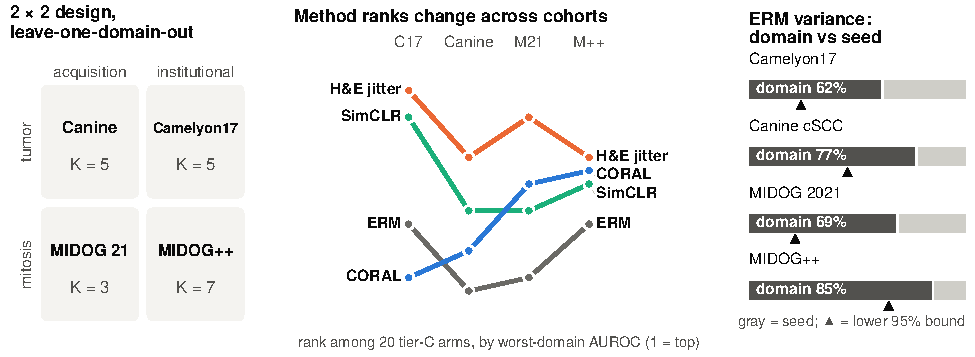
\includegraphics[width=\textwidth]{graphical_abstract}
%\end{graphicalabstract}

%%% Highlights (mandatory; 3-5 bullets, each <= 85 characters incl. spaces).
%%% Also supplied as a separate editable file: submission/highlights.txt.
\begin{highlights}
\item Models trained once can work at unseen sites, but no recipe wins everywhere
\item Judge a pathology model by its worst hospital or scanner, not by its average
\item Default recipe: fine-tune a pathology foundation model with color jitter
\item A site acceptance test checks each new hospital with a few local labels
\item At standard scale it needs about half the labels, with $\le$2.1\% false acceptance
\end{highlights}

%%% Keywords (at most 6; American spelling; no multi-concept "and"/"of" terms).
\begin{keywords}
Computational pathology \sep Domain generalization \sep Multi-site validation \sep
Foundation models \sep Test-time adaptation \sep Evaluation methodology
\end{keywords}

\maketitle

%%% ---------------------------- Main text ---------------------------
%% Introduction (MedIA revision, v2 pipeline). Numbers follow Section 5 (sections/results.tex).
\section{Introduction}
\label{sec:intro}

Deep networks for histopathology often lose accuracy when they are applied to
slides from a laboratory, scanner or patient population they were not trained
on. Staining protocols, scanners and tissue handling differ between sites, and
networks pick these differences up: the submitting site of a TCGA slide can be
predicted from the image, and this signal biases downstream predictions
\citep{howard2021site}. Color differences between laboratories degrade
classifiers on unseen laboratories \citep{tellez2019stain}, and mitotic-figure
detectors deteriorate on new scanners and tumor types
\citep{aubreville2023midog,aubreville2024midog2022}. The problem is not
specific to pathology; most externally validated radiology models also perform
worse on external data \citep{yu2022external}.

For practitioners, the goal is a model that is trained once and then works at
every hospital where it is used, without collecting labels or retraining at
each new site. Many remedies promise this: stain normalization and color
augmentation, domain-generalization (DG) objectives, self-supervised
pre-training, test-time adaptation and, most recently, pathology foundation
models. To choose between them, practitioners need evidence that can tell a
real difference from noise.
That is harder than it looks. Benchmarks with a single official test site,
such as Camelyon17-WILDS, evaluate every method on one domain, and ERM accuracy
on that domain has a standard deviation of 6.4 points across ten seeds
\citep{koh2021wilds}.
Across DG benchmarks, ERM is hard to beat once every method is tuned and
evaluated under the same protocol \citep{gulrajani2021domainbed}. Rankings in
biomedical image analysis challenges are sensitive to the test data and the
ranking scheme \citep{maierhein2018rankings}. A reported gain can thus reflect
the chosen test site, the seed or the tuning budget as much as the method.

This study began with such a gain. In an earlier version of this work, a
single Camelyon17 test hospital suggested that self-supervised pre-training and
sharpness-aware minimization were synergistic. Each method alone was worse than
ERM, and together they were better. Repeating the runs and holding out every
hospital in turn reversed the sign of this interaction at most hospitals
(Section~\ref{sec:casestudy}). The same earlier version argued that the type of
shift, scanner-only or institutional, decides which method works best. That
argument rested on two cohorts that differed in task as well as in shift type,
and an audit of our code found defects in several method implementations. We
therefore rebuilt the study around six questions:
\begin{enumerate}
  \item How much of the variance of a held-out score comes from the choice of
    held-out domain, and how much from run-to-run noise?
  \item With the few domains that pathology cohorts provide, can realistic
    differences between methods be detected at all?
  \item How stable are method rankings within a cohort?
  \item Do rankings carry over between cohorts that share the task, or between
    cohorts that share the type of shift?
  \item Which choices give a model the best chance of working at an unseen site
    without retraining?
  \item How can a practitioner decide, with few local labels, whether a trained
    model is good enough at a particular new site?
\end{enumerate}

To answer them, we use a \emph{domain-complete, seed-replicated} protocol.
Every domain of a cohort is the test domain of one leave-one-domain-out fold,
every method is run at several seeds under one fixed training budget, and
hyperparameters and checkpoints are selected without test data. We analyze the
results with a random-effects decomposition into between-domain and
between-run variance with interval estimates, paired contrasts with a
fold-dependence sensitivity analysis, a power calculation based on the
variance of the paired difference, and bootstrap intervals for ranks and for
rank agreement between cohorts. We apply the protocol to four public cohorts
arranged in a $2\times2$ design. Two tumor-classification cohorts and two
mitotic-figure cohorts each pair an acquisition-only shift (scanners within
one laboratory) with an institutional shift (hospitals or tumor types).
We evaluate up to 21 arms at two model scales, a compact CNN and ImageNet
ResNet-50, together with frozen and fine-tuned pathology foundation models,
in 4,778 training runs. No model is ever trained on labeled data from its test
site, and apart from the test-time adaptation arms, which use unlabeled test
images, every result measures how a model trained once performs, unchanged, at
a site it has never seen.

Our contributions are:
\begin{itemize}
  \item an empirical-Bayes \emph{site acceptance test} that decides whether a
    trained model reaches a target AUROC at a new site. It combines the
    between-site spread of the development results with a small labeled sample
    from the new site, plans the number of labels in advance, and is validated
    on every held-out site of the study (Sections~\ref{sec:sat}
    and~\ref{sec:results-sat});
  \item a six-step, evidence-graded roadmap for practitioners who need models
    that work across hospitals and scanners without retraining, covering the
    target definition, data collection, training recipe, label-free adaptation
    at a new site, validation and site acceptance
    (Section~\ref{sec:roadmap});
  \item an evaluation protocol and a set of diagnostics for distribution shift
    in multi-domain pathology cohorts, with the code, the fold definitions and
    every per-run record released so that each table and figure can be
    regenerated;
  \item a $2\times2$ task-by-shift study at two model scales, with
    domain-generalization objectives, stain and color methods,
    self-supervision, test-time adaptation, pathology foundation models and
    two controls for self-supervision, all tuned per fold;
  \item an external reference point for the variance decomposition, computed
    from DomainBed's published per-environment results;
  \item two negative results reported in full: a single-hospital synergy
    claim that does not survive the protocol, and a single-institution cohort
    that cannot support domain claims.
\end{itemize}

The main findings are these. Without retraining, the best standard-scale
method of each cohort reached a worst-site AUROC of 0.884 to 0.986, against
0.534 to 0.895 for ERM, but no method was best everywhere. For most arms, the held-out domain accounts for
most of the variance of a single run (median ICC 0.72--0.95), and the worst
domain differs between methods. After correction for multiple comparisons, no
standard-tier method beats ERM on any cohort. Even a mean gain of 0.145 AUROC
that holds at every domain is not significant with five domains, and detecting
a gain of 0.05 on the tumor cohorts would need between 7 and 53 domains. Under
the primary selection rule, none of the six DG objectives ranks in the top five
on any cohort. At the standard
tier, method rankings agree more between cohorts that share a task than
between cohorts that share a shift type. With one cohort per cell this is a
description, not a proof, and the compact tier does not clearly show it. Fine-tuned
pathology foundation models with color augmentation were the most reliable
choice on average, and re-estimating batch-normalization statistics at the new
site, which needs no labels and no weight updates, helped mainly under severe
scanner shift. Implementation choices such as per-tile versus per-slide
stain estimation, and the learning rate of a pretrained encoder, change
results as much as the choice of method. Finally, the development results
alone would have accepted 8.6\% of the sites that fell below an AUROC of 0.80.
At standard scale, the site acceptance test kept false acceptance at or below
2.1\% and, for targets of 0.80 and 0.85, reached the same power as local labels
alone with about half as many labels.

Section~\ref{sec:related} reviews related work. Section~\ref{sec:protocol}
defines the protocol, the statistics and the site acceptance test, and
Section~\ref{sec:setup} the cohorts, models and arms. Section~\ref{sec:results} reports the results.
Section~\ref{sec:discussion} discusses them, presents the roadmap
(Section~\ref{sec:roadmap}) and the two case studies, and lists the
limitations.

%% Related work (MedIA revision). Every factual statement about a cited paper is
%% traced to its source in sections/related_claims.md.
\section{Related work}
\label{sec:related}

\subsection{Site and center effects}
\label{sec:related-site}

Performance loss at institutions not seen in training is documented across
medical imaging. \citet{zech2018variable} trained pneumonia classifiers on chest
radiographs from three hospital systems. Internal performance exceeded external
performance in three of five comparisons, and for two of the systems the
networks identified the system a radiograph came from with more than 99.9\%
accuracy. In a systematic review of 86 externally validated radiology
algorithms, 81\% performed worse on external data and 24\% lost at least 0.10
on the unit scale \citep{yu2022external}. In histopathology,
\citet{howard2021site} showed that the submitting site of TCGA slides can be
identified by deep networks even after common color normalization and
augmentation. These site signatures biased the accuracy of survival, mutation
and stage prediction. The authors proposed splits in which no site contributes
to both training and validation. \citet{stacke2019closer} proposed a
model-specific distance between domains, computed in the learned
representation. \citet{stacke2021measuring} developed it into the
\emph{representation shift} and showed that it correlates highly with the drop
in performance across many types of domain shift. These studies show that site
effects exist and can be detected, but not how much of the spread in reported
performance they account for relative to the training method. Our variance
decomposition estimates this.

Mitotic-figure detection has been studied directly under domain shift. The
MIDOG~2021 challenge trained on 200 breast cancer cases from four scanners (one
of them without labels) and
tested on 100 cases from four scanners, two of which were not seen in training.
The winning method reached an F1 score of 0.748 \citep{aubreville2023midog}.
MIDOG~2022 extended the shift across tumor types, laboratories and species
(as its title states) and evaluated nine methods on ten independent domains. Domain characteristics
absent from the training data (a new species, a new cell morphology and a new
scanner) led to small but significant drops in performance
\citep{aubreville2024midog2022}. The method that won both editions combined a
two-stage detector with domain-generalization measures
\citep{jahanifar2024mitosis}. MIDOG++ \citep{aubreville2023midogpp} released
503 images of seven tumor types and found that leave-one-domain-out training
generalized considerably better than training on a single domain. The
multi-scanner canine cutaneous squamous cell carcinoma dataset
\citep{wilm2023canine} digitized the same slides with five scanners, which
isolates the acquisition shift. We use these cohorts, but our question is not
the challenges' question of which detector is best. We ask how much of a
comparison between methods is decided by the domains themselves.

\subsection{Domain generalization benchmarks and protocols}
\label{sec:related-dg}

Leave-one-domain-out evaluation with repeated runs is established practice in
domain generalization (DG); \citet{zhou2023domain} survey the field. DomainBed
\citep{gulrajani2021domainbed} evaluated fourteen algorithms on seven
multi-domain datasets. It trained on the remaining domains for every choice of held-out test
domain, and it repeated the whole study three times, redrawing hyperparameters,
weight initializations and data splits. The authors argued that a DG algorithm
without a model-selection rule is incomplete. They compared three rules:
validation data pooled from the training domains, leave-one-domain-out
cross-validation over the training domains, and an oracle validation set drawn
from the test domain. With training-domain or oracle selection, no algorithm
improved on the average accuracy of empirical risk minimization (ERM) by more
than one point, and the authors found no improvement over ERM statistically
significant. Under leave-one-domain-out selection, however, CORAL led ERM by
1.8 points \citep[Table~3]{gulrajani2021domainbed}.
Training-domain validation also outperformed leave-one-domain-out
cross-validation across multiple datasets and algorithms.

WILDS \citep{koh2021wilds} made Camelyon17 \citep{bandi2019camelyon17} a DG
benchmark with three training hospitals, one out-of-distribution (OOD)
validation hospital and one test hospital. The test hospital was chosen because
its patches were the most visually distinctive. ERM test accuracy had a
standard deviation of 6.4 points over ten seeds, and CORAL, IRM and GroupDRO
performed comparably to or worse than ERM. WILDS therefore asks for ten seeds
per Camelyon17 submission and warns that so few test domains invite overfitting
to them. WILDS~2.0 \citep{sagawa2022extending} added unlabeled patches from the
training, validation and test hospitals. On Camelyon17, ERM reached 70.8\% OOD
accuracy without data augmentation and 82.0\% with it. SwAV pre-training on
unlabeled target-hospital patches reached 91.4\% (standard deviation 2.0) and
Noisy Student reached 86.7\%. CORAL, DANN, Pseudo-Label and FixMatch all fell
below augmented ERM \citep[Table~2]{sagawa2022extending}. These figures come
from one held-out hospital. The best arm also sees unlabeled images from that
hospital, so it is unsupervised adaptation rather than DG.
\citet{wiles2022fine} distinguished spurious correlation, low-data drift and
unseen data shift, and trained more than 85,000 models covering 19 methods on
six datasets, Camelyon17 among them. Pre-training and augmentation often helped
substantially, but the best methods differed across datasets and shifts. On
Camelyon17, color jitter hurt performance, and pre-training was not the best
choice under unseen data shift.

We adopt leave-one-domain-out evaluation and training-domain model selection
from this literature and claim neither as new. Our contribution is diagnostic.
We decompose performance into between-domain and between-run variance with
interval estimates, and we analyze how stable method rankings are across
held-out domains and cohorts. We use a factorial cohort design that crosses task
(tumor versus mitotic figure) with shift type (institutional versus
acquisition-only). Ranking agreement can then be compared between cohorts that
share a task and cohorts that share a shift type.

\subsection{Stain normalization and augmentation}
\label{sec:related-stain}

Differences in staining between laboratories degrade networks applied to
slides from an unseen laboratory \citep{tellez2019stain}.
\citet{reinhard2001color} transferred color by matching per-channel means and
standard deviations in the decorrelated $l\alpha\beta$ space. Color
deconvolution \citep{ruifrok2001deconvolution} separates up to three stains in
RGB images using stain-specific absorption, and it is the basis of HED-space
augmentation \citep{tellez2019stain}. \citet{macenko2009} estimate the stain
vectors of each slide from its optical densities. Pixels are projected onto the
plane of the two leading singular vectors, the vectors are taken at robust
angular extremes, and per-stain intensities are rescaled to a common
pseudo-maximum. \citet{vahadane2016structure} factorize images into sparse,
non-negative stain density maps and recombine them with a target image's stain
color basis. StainGAN \citep{shaban2019staingan} learns the mapping with a
CycleGAN-style model, so no single reference slide has to be chosen. Instead of normalizing,
\citet{tellez2018whole} perturbed the hematoxylin and eosin channels directly
and, together with ensembling, obtained a stain-invariant mitosis detector.
Across four tasks and nine laboratories, \citet{tellez2019stain} found HSV or
HED color augmentation essential. The top-ranked configuration used no
normalization, although normalization made classifiers less sensitive to the
choice of augmentation. Normalization also leaves site information in place
\citep{howard2021site}. We therefore evaluate per-slide Macenko normalization,
a per-tile variant, H\&E jitter and their combination as separate arms.

\subsection{Self-supervision and pathology foundation models}
\label{sec:related-fm}

\citet{ciga2022ssl} pre-trained SimCLR on 57 unlabeled histopathology datasets.
Linear classifiers on these features beat ImageNet features by more than 28\%
in F1 on average. \citet{kang2023benchmarking} compared MoCo~v2,
SwAV, Barlow Twins and DINO pre-trained on 19 million patches from 20,994 TCGA
slides, and domain-aligned pre-training outperformed ImageNet pre-training in
both linear and fine-tuning evaluation. Foundation models extend this further:
\begin{itemize}
  \item CTransPath, a convolutional network combined with a multi-scale Swin
    Transformer \citep{wang2022ctranspath};
  \item Phikon, an iBOT ViT-Base trained on more than 40 million images from 16
    cancer types \citep{filiot2023phikon};
  \item UNI, trained on more than 100 million images from over 100,000
    whole-slide images (WSIs) covering 20 tissue types \citep{chen2024uni};
  \item CONCH, trained on more than 1.17 million image--caption pairs
    \citep{lu2024conch};
  \item Virchow, a 632-million-parameter ViT trained with DINOv2 on about
    1.5 million WSIs \citep{vorontsov2024virchow};
  \item Prov-GigaPath, trained on 1.3 billion tiles from 171,189 slides from a
    network of 28 cancer centers \citep{xu2024gigapath}.
\end{itemize}

Scale does not by itself remove center effects. \citet{komen2024batch} found
hospital signatures in foundation-model embeddings that dominated feature-space
distances and were not removed by stain normalization. All ten public
foundation models evaluated by \citet{dejong2025unrobust} encoded the medical
center strongly. Only one had a robustness index above one, meaning that
biological features outweighed center features, and then only slightly.
The PathoROB benchmark found robustness deficits in all 20 models it evaluated
\citep{komen2026robust}. More robust models, vision--language alignment and
post-hoc robustification reduced, but did not eliminate, the risk of the
resulting downstream errors. Our analysis is complementary. We measure how the
downstream performance of frozen and fine-tuned pathology encoders
\citep{kang2023benchmarking} varies across held-out domains, under the same
protocol and diagnostics as every other arm.

\subsection{Test-time adaptation}
\label{sec:related-tta}

AdaBN adapts a trained network without labels by replacing its
batch-normalization (BN) statistics with target-domain statistics, and it adds
no parameters \citep{li2017adabn}. \citet{schneider2020bn} showed that
re-estimating BN statistics on corrupted images improved ImageNet-C robustness
for 25 architectures, and argued that adapted results should be reported in OOD
evaluations. Prediction-time BN improved accuracy and calibration under
covariate shift, but its results were mixed when combined with pre-training and
weaker under more natural shifts \citep{nado2020bn}. TENT \citep{wang2021tent}
minimizes prediction entropy online, updating normalization statistics and
channel-wise affine parameters on each batch. Because these methods estimate
statistics from test batches, which depend on batch composition, our protocol
shuffles the test stream with a fixed seed before any adaptation.

\subsection{Variance, rankings and statistical reporting}
\label{sec:related-stats}

Data sampling, parameter initialization and hyperparameter choice each have a
marked effect on benchmark results \citep{bouthillier2021variance}, and
test-set scores alone do not settle which model is best \citep{dodge2019show}.
In biomedical image analysis challenges, an algorithm's rank is generally not
robust to the test data, the ranking scheme or the annotators
\citep{maierhein2018rankings}. challengeR provides bootstrap analyses of ranking
stability \citep{wiesenfarth2021challenger}. \citet{varoquaux2018cv} showed
that cross-validation error bars are large (about $\pm 10\%$ with 100 samples)
and that the standard error across folds strongly underestimates them. In two
Kaggle medical-imaging challenges with test sets below 1,000 cases, the
difference between the public and private leaderboards was larger than the gap
between the winner and the top-10\% entry \citep{varoquaux2022failures}. Any variance estimator computed only from the
results of a cross-validation experiment is biased, and ignoring
training-set variability can make an algorithm look significantly better than
it is \citep{nadeau2003inference}. Cross-validation estimates the average error
of models fit to other training sets from the same population (proved for
least-squares linear models), and the correlation between folds makes
the usual intervals too narrow \citep{bates2023cv}. Leave-one-domain-out
designs are an extreme case. There are few folds ($K=3$ to $7$ here), the folds
share training domains, and the held-out domain is both a nuisance factor and
the quantity of interest. We therefore report between-domain and between-run
variance components with intervals and run a fold-dependence sensitivity
analysis on paired contrasts. We also give bootstrap intervals for method ranks
(over seeds and over domains) and for Kendall's $\tau$ between cohort rankings.

%% Evaluation protocol (MedIA revision, v2 pipeline).
%% Every implementation detail below is taken from src/v2/ (run_v2.py, arms.py,
%% select_hparams.py, stats_v2.py, analyze_v2.py); see the provenance list kept
%% with the revision notes.
\section{Evaluation protocol}
\label{sec:protocol}

A cohort has $K$ domains, and fold $t$ holds out domain $t$ for testing. Every
arm (a training method or a test-time procedure) is run in every fold with
several seeds. The cohorts, models and arms are described in
Section~\ref{sec:setup}.

\subsection{Leave-one-domain-out design}
\label{sec:protocol-lodo}

Leave-one-domain-out evaluation is standard in domain generalization
\citep{gulrajani2021domainbed}, and Camelyon17-WILDS adds a held-out validation
hospital \citep{koh2021wilds}. We follow both. On Camelyon17, the canine
cohort and MIDOG++, fold $t$ also holds out domain $(t-1)\bmod K$ as an
out-of-distribution (OOD) validation domain and trains on the remaining $K-2$
domains. MIDOG~2021 has three labeled scanners, so each fold trains on two and
has no OOD validation domain. Every domain is the test domain of exactly one
fold, so the evaluation is \emph{domain-complete}: no single test domain is
privileged. In every training domain, an in-distribution (ID) validation split
is held out that is disjoint from training in its groups (patients, slides or
images; Section~\ref{sec:setup-cohorts}). The study adds four elements to this
design.

\paragraph{Seed replication} Every arm is run in every fold with five seeds at
the compact tier and three at the standard tier
(Section~\ref{sec:setup-models}). The seed fixes the initialization of
randomly initialized layers, the batch order, the augmentation draws and the
order of the test stream for test-time adaptation. All arms use the same seed
values.

\paragraph{Fixed step budget} Every fine-tuned arm is trained for 1,200 steps
with batch size 128 and a cosine learning-rate schedule. It is evaluated at
ten checkpoints, at steps $\mathrm{round}(kn/10)$ for $k=1,\dots,10$ and a
budget of $n$ steps. The only exception is the compute-matched control
(Section~\ref{sec:setup-arms}), which needs a larger budget by design. With a
fixed budget, schedule length and early stopping cannot confound method
comparisons.

\paragraph{All model-selection rules} At each checkpoint we evaluate the ID
validation, OOD validation and test splits. Four rules select a checkpoint by
the maximum area under the ROC curve (AUROC) on their selection split, with ties
going to the earliest checkpoint:
\begin{enumerate}
  \item \emph{training-domain (ID) validation}, the primary rule
    \citep[DomainBed's default;][]{gulrajani2021domainbed}, available in every
    cohort;
  \item \emph{leave-one-domain-out validation} on the OOD validation domain
    (Camelyon17, canine, MIDOG++);
  \item \emph{last}, the final checkpoint;
  \item \emph{oracle}, the best test AUROC, reported only as an upper bound.
\end{enumerate}
All four rules use the same ten checkpoints of the same runs, so any
difference between them comes from selection alone.

\paragraph{Per-fold hyperparameter selection} Hyperparameters are tuned with
seed~0 on the grids of Table~\ref{tab:arms}. Every fold keeps the configuration
with the highest ID-validation AUROC at the ID-selected checkpoint of its own
tuning run. Diverged runs are excluded unless every configuration diverged, and
test data are never used. We do not average ID-validation AUROC over folds,
because doing so leaks test-domain labels. The test domain of fold $t$ is a
training domain of the other folds, except for fold $t+1$ when a validation
domain exists. The ID-validation splits of those folds therefore contain
labeled patches of domain $t$. In every cohort, some of these patches are
pixel-identical to rows of fold $t$'s test set.
Averaging would thus let fold $t$'s test labels influence the hyperparameters
reported for fold $t$. At the standard tier, the base learning rate is selected
first, and the method grids are then run at each fold's selected rate. The
Barlow Twins fine-tunes have their own rate grid (Section~\ref{sec:setup-optim}).

\subsection{Reported quantities}
\label{sec:protocol-metrics}

Let $y_{ts}$ be the test AUROC (the primary metric) of one arm in fold $t$
with seed $s=1,\dots,n_t$ under a given selection rule, and
$\bar y_t=n_t^{-1}\sum_s y_{ts}$. For every arm, cohort, tier and rule we report
\begin{align}
  \text{worst domain:}\quad & \min_t \bar y_t, \label{eq:worst}\\
  \text{across-domain SD:}\quad & s_{\bar y}=\Big[\tfrac{1}{K-1}\textstyle\sum_t(\bar y_t-\hat\mu)^2\Big]^{1/2},
     \label{eq:sdacross}\\
  \text{mean:}\quad & \hat\mu = \tfrac{1}{K}\textstyle\sum_t \bar y_t,\qquad
     \hat\mu \pm t_{0.975,\,K-1}\, s_{\bar y}/\sqrt{K}. \label{eq:mean}
\end{align}
With balanced seeds, the interval in \eqref{eq:mean} is exact under model
\eqref{eq:oneway}, since $\operatorname{Var}(\bar y_t)=\sigma_D^2+\sigma_R^2/n$
for every domain. Percentile bootstrap intervals \citep{efron1993bootstrap}
are supplementary only, because the domain bootstrap under-covers for $K\le7$.
Calibration is reported as the expected calibration error
\citep{naeini2015ece,guo2017calibration}, with 15 equal-width bins $B_b$ on the
confidence of the predicted class (decision threshold 0.5):
\begin{equation}
  \mathrm{ECE}=\sum_{b=1}^{15}\frac{|B_b|}{N_{\text{test}}}\,
  \big|\operatorname{acc}(B_b)-\operatorname{conf}(B_b)\big|,
  \label{eq:ece}
\end{equation}
summarized by its mean and maximum over domains.

\subsection{Variance decomposition}
\label{sec:protocol-variance}

For one arm on one cohort we fit the one-way random-effects model
\begin{equation}
  y_{ts}=\mu+b_t+e_{ts},\qquad b_t\sim\mathcal N(0,\sigma_D^2),\quad
  e_{ts}\sim\mathcal N(0,\sigma_R^2),\qquad s=1,\dots,n_t,
  \label{eq:oneway}
\end{equation}
with all terms independent. Seeds are nested within domains: seed $s$ in
folds $t$ and $t'$ denotes different runs on different training sets, so no
crossed seed effect is fitted. $\sigma_D$ is the between-domain and $\sigma_R$
the between-run SD. With $N=\sum_t n_t$, between- and within-domain mean
squares $\mathrm{MSB}=\sum_t n_t(\bar y_t-\bar y)^2/(K-1)$ and
$\mathrm{MSW}=\sum_{t,s}(y_{ts}-\bar y_t)^2/(N-K)$, and
$n_0=(N-\sum_t n_t^2/N)/(K-1)$ ($n_0=n$ for balanced data), the ANOVA
estimators \citep{searle1992variance} are
\begin{equation}
  \hat\sigma_R^2=\mathrm{MSW},\qquad
  \hat\sigma_D^2=\max\{(\mathrm{MSB}-\mathrm{MSW})/n_0,\,0\},\qquad
  \widehat{\mathrm{ICC}}=\frac{\mathrm{MSB}-\mathrm{MSW}}{\mathrm{MSB}+(n_0-1)\,\mathrm{MSW}},
  \label{eq:anova}
\end{equation}
where $\mathrm{ICC}=\sigma_D^2/(\sigma_D^2+\sigma_R^2)$ is ICC(1)
\citep{shrout1979icc,mcgraw1996icc}, reported truncated at 0. Restricted
maximum likelihood (REML) estimates \citep{patterson1971reml} are obtained by
profiling out $\sigma_R^2$ and minimizing over $\gamma=\sigma_D^2/\sigma_R^2\ge0$,
with the boundary $\gamma=0$ checked explicitly. They coincide with ANOVA for
balanced data with a positive estimate.

\paragraph{Intervals and boundary estimates} We report the exact $F$-based
95\% interval for the ICC, the exact $\chi^2$ interval for $\sigma_R$ and the
modified large-sample interval for $\sigma_D$
\citep{searle1992variance,mcgraw1996icc,burdick1992confidence}. With $K\le7$,
$\hat\sigma_D$ is often at or near zero, so we also report a Bayesian grid
posterior under weakly informative half-normal and half-Cauchy priors (scale
0.1 AUROC) \citep{gelman2006prior}, with one-sided intervals $[0,q_{0.95}]$ at
the boundary. The formulas are in Supplementary
Section~\ref{S-sup:protocol}.

\paragraph{The ICC as a diagnostic} The ICC is the share of an arm's
single-run variance that is due to which domain is held out. Near one, the
choice of domains dominates. Near zero, run-to-run noise is as large as the
differences between domains, and a single-seed result says little about a
domain. The ICC is conditional on arm, cohort, metric, selection rule and the
domains at hand, and with $K\le7$ its intervals are wide. It tells us where the
variance of a reported number comes from. It is not a quality standard, and we
set no threshold for it. As an external reference point we apply the same
estimators to DomainBed's published per-environment results
\citep{gulrajani2021domainbed}. The mean $\pm$ standard error over three
trials is converted to an SD with the convention of DomainBed's released code
(Supplementary Section~\ref{S-app:domainbed}).

\subsection{Paired contrasts and fold dependence}
\label{sec:protocol-contrasts}

Each arm is compared with ERM of the same tier and cohort through
$d_t=\bar y^{a}_t-\bar y^{\text{ERM}}_t$. We report $\bar d$, the interval
$\bar d\pm t_{0.975,K-1}s_d/\sqrt K$, the two-sided $p$-value and the number of
improved domains. The $p$-values are Holm-adjusted over all arms compared with
ERM within a cohort, tier and selection rule \citep{holm1979}.

The folds of a leave-one-domain-out design share training domains, so the
$d_t$ are not independent \citep{nadeau2003inference,bates2023cv}. Let $T_i$ be
the set of training domains of fold $i$ and
$O_{ij}=|T_i\cap T_j|/\sqrt{|T_i||T_j|}$ the overlap of folds $i$ and $j$. As
a sensitivity analysis we assume a working correlation
$\operatorname{corr}(d_i,d_j)=R_{ij}=\rho\,O_{ij}$ for $i\ne j$
($R_{ii}=1$). Under this assumption
$\operatorname{Var}(\bar d)=\sigma^2\,\mathbf 1^\top R\mathbf 1/K^2$, and the
sample variance is biased downward,
$\mathbb E[s_d^2]=\sigma^2(1-\bar r)$, where $\bar r$ is the mean off-diagonal
element of $R$. The corrected standard error and the effective number of folds
are then
\begin{equation}
  \widehat{\mathrm{SE}}_\rho(\bar d)=\Big[\frac{s_d^2}{1-\bar r}\,
  \frac{\mathbf 1^\top R\mathbf 1}{K^2}\Big]^{1/2},\qquad
  K_{\text{eff}}=\frac{K^2}{\sum_{i,j}R_{ij}},
  \label{eq:keff}
\end{equation}
with $t_{K-1}$ quantiles, in the spirit of the corrected resampled $t$
statistic of \citet{nadeau2003inference}. Because $\rho$ cannot be estimated
from $K$ folds, we report $\rho\in\{0,0.25,0.5,1\}$. For our designs,
$K_{\text{eff}}=3.33$, 2.50 and 1.67 at $\rho=0.25$, 0.5 and 1 for Camelyon17
and the canine cohort ($K=5$); 3.50, 2.33 and 1.40 for MIDOG++ ($K=7$); and
2.40, 2.00 and 1.50 for MIDOG~2021 ($K=3$).

\subsection{Power}
\label{sec:protocol-power}

Power for a paired comparison depends on the variance of the paired
difference, not on either arm's between-domain SD. Writing
$y^{a}_{ts}=\mu_a+b_t+(ab)_{t}+e^{a}_{ts}$ and
$y^{\text{ERM}}_{ts}=\mu_{\text{ERM}}+b_t+e^{\text{ERM}}_{ts}$, the domain
effect $b_t$ cancels, and with $s$ seeds per arm
\begin{equation}
  \sigma_\Delta^2(s)=\operatorname{Var}(d_t)=\sigma_{DA}^2+\sigma_{R,\Delta}^2/s,
  \qquad \sigma_{R,\Delta}^2=\operatorname{Var}(e^{a}_{ts}-e^{\text{ERM}}_{ts}),
  \label{eq:diffvar}
\end{equation}
where $\sigma_{DA}^2$ is the domain-by-arm interaction variance. Because all
arms share seed values, their run noise may be correlated, so
$\sigma^2_{R,\Delta}$ is estimated as the pooled within-domain variance of the
per-seed differences $y^{a}_{ts}-y^{\text{ERM}}_{ts}$, which is unbiased either
way, and $\hat\sigma_{DA}^2=\max\{s_d^2-\hat\sigma^2_{R,\Delta}h,0\}$ with
$h=K^{-1}\sum_t n_t^{-1}$. If seed sets are not aligned, we use
$\hat\sigma^2_{R,\Delta}=\mathrm{MSW}_a+\mathrm{MSW}_{\text{ERM}}$ and
$\hat\sigma_{DA}^2=\max\{s_d^2-\mathrm{MSW}_a h_a-\mathrm{MSW}_{\text{ERM}}h_{\text{ERM}},0\}$.
The power of the two-sided paired $t$ test over $K$ domains to detect a mean
difference $\delta$ is
\begin{equation}
  1-\beta(K)=\Pr\big(|T_{K-1}(\lambda)|>t_{1-\alpha/2,\,K-1}\big),\qquad
  \lambda=\frac{\delta\sqrt{K_{\text{eff}}}}{\sigma_\Delta(s)},
  \label{eq:power}
\end{equation}
where $T_{K-1}(\lambda)$ is noncentral $t$ with $K-1$ degrees of freedom and
$K_{\text{eff}}=K$ for independent folds. We report the smallest $K$ that
reaches 80\% power at $\alpha=0.05$, for
$\delta\in\{0.02,0.05,0.10,0.20\}$ AUROC and $s\in\{1,3,5,10\}$. For
$\rho>0$, $\sigma_\Delta$ is first divided by $\sqrt{1-\bar r_{\text{obs}}}$
(the bias correction of \eqref{eq:keff} for the observed design). The primary
\emph{ratio} mode then holds the observed inflation $K/K_{\text{eff}}$ fixed as
$K$ grows. The \emph{design} mode uses $K_{\text{eff}}$ of a hypothetical
$K$-domain design, which levels off near $1/\rho$ because training sets overlap
more as $K$ grows, so some targets are unreachable.

\subsection{Rank stability and the task-by-shift decomposition}
\label{sec:protocol-ranks}

Within a cohort, arms are ranked by worst-domain \eqref{eq:worst} and by mean
AUROC, with 95\% percentile rank intervals and the probability of ranking first
from 5,000 bootstrap replicates. Two resampling schemes are used: seeds within
each (arm, domain) cell, and domains with one shared draw for all arms.
Agreement between two cohorts' rankings is Kendall's $\tau_b$ over their common
arms \citep{kendall1938}, with a 95\% interval from 2,000 seed-bootstrap
replicates and a $p$-value against independent orderings. Of the six cohort
pairs, two share the task, two the shift type and two neither. We report the
mean worst-domain $\tau_b$ per class and bootstrap intervals of the differences, which are
descriptive.

\paragraph{Arm-by-cohort interaction} For the $A$ arms that are run in all
four cohorts, let $G_{cta}=\bar y^{a}_{ct}-\bar y^{\text{ERM}}_{ct}$ be the
gain of arm $a$ over ERM in domain $t$ of cohort $c$. Each (cohort, domain) row
is centered across arms, $E_{cta}=G_{cta}-A^{-1}\sum_{a'}G_{cta'}$, removing
the domain's average gain. Whether the centered profiles differ between cohorts
is tested with domains as replicates, using a studentized Welch--James statistic
and a wild bootstrap that multiplies whole residual rows by Rademacher signs
(10,000 replicates). This keeps each cohort's variance and the correlation
between arms.

\paragraph{Task, shift and task $\times$ shift} Task and shift type are
constant within a cohort, so they can only be assessed with the cohort as the
unit. Let $\mathbf m_c\in\mathbb R^A$ be the mean of the centered rows of
cohort $c$, with equal weight for every cohort, and let $s^{f}_c=\pm1$ code
cohort $c$ for factor
$f\in\{\text{task},\text{shift},\text{task}\times\text{shift}\}$, with
$s^{\text{task}\times\text{shift}}_c=s^{\text{task}}_c s^{\text{shift}}_c$.
Because the four cohorts form a $2\times2$ design with one cohort per cell, the
between-cohort interaction sum of squares splits exactly into three orthogonal
contrasts:
\begin{equation}
  \sum_{c}\|\mathbf m_c-\bar{\mathbf m}\|^2
  =\sum_{f}\mathrm{SS}_f,\qquad
  \mathrm{SS}_f=\|\mathbf L_f\|^2,\quad
  \mathbf L_f=\tfrac12\sum_c s^{f}_c\,\mathbf m_c .
  \label{eq:2x2}
\end{equation}
We report each $\mathrm{SS}_f$ and its fraction of the total, and the rank
of the task and shift splits among the three possible two-versus-two splits of
four cohorts. A cohort-level permutation $p$-value equals rank$/3$ and cannot
be below $1/3$. We also give an approximate test $F_f=\mathrm{SS}_f/\mathrm{SS}_{\text{task}\times\text{shift}}$
on $(A-1,A-1)$ degrees of freedom for $f\in\{\text{task},\text{shift}\}$. It
treats the cohort-level deviations as independent and spherical across arms.
Its error term has only $A-1$ degrees of freedom and absorbs any genuine
task-by-shift pattern. With four cohorts, this decomposition describes the
interaction. It cannot show that rankings are organized by task or by shift
type, and we do not claim that they are.

\subsection{A site acceptance test for new sites}
\label{sec:sat}

The diagnostics above describe a method across sites. A practitioner who is
about to use one trained model at a new hospital or scanner needs a decision
for that site: is the model's AUROC there at least a target $T$? We propose an
empirical-Bayes site acceptance test that combines the development evidence
with a small labeled sample from the new site.

\paragraph{Development prior} Let $z_{sr}=\operatorname{logit}(y_{sr})$ be the
test AUROC of run $r$ of the method at development site $s$ on the logit scale,
for $K'$ held-out development sites with $n$ runs each. Under model
\eqref{eq:oneway} on this scale, with a flat prior on $\mu$ and independent
half-Cauchy priors on $\sigma_D$ and $\sigma_R$, the AUROC of one run at a new
site has, on the logit scale, the posterior predictive distribution
\begin{equation}
  \theta_{\text{new}}\mid\sigma_D,\sigma_R,\mathbf z\ \sim\
  \mathcal N\!\Big(\bar z,\ \sigma_D^2+\sigma_R^2+\frac{\sigma_D^2+\sigma_R^2/n}{K'}\Big),
  \label{eq:sat-prior}
\end{equation}
integrated over the grid posterior of $(\sigma_D,\sigma_R)$, where $\bar z$ is
the grand mean. The result is a scale mixture of normal distributions centered
at $\bar z$. Its spread grows with the between-site SD and shrinks only slowly
with $K'$, so few or heterogeneous development sites give a vague prior. The
half-Cauchy scale is 0.5 on the logit scale (about 0.06 AUROC at an AUROC of
0.85).

\paragraph{Local evidence} At the new site, $m$ patches are labeled. Their AUROC
$a_m$ (with a continuity correction that keeps it inside $(0,1)$) gives
$\hat z_m=\operatorname{logit}(a_m)$ with variance
$v_m=\operatorname{Var}(a_m)/\{a_m(1-a_m)\}^2$, where $\operatorname{Var}(a_m)$
is the Hanley--McNeil variance for the observed numbers of positives and
negatives. Each mixture component is updated conjugately with
$\hat z_m\sim\mathcal N(\theta,v_m)$, and the component weights are updated by
their marginal likelihoods.

\paragraph{Decision} The site is accepted if
$P(\theta\ge\operatorname{logit}T\mid\mathbf z,\hat z_m)\ge 1-\alpha$, with
$\alpha=0.05$. The posterior also gives a point estimate and a credible interval
for the site's AUROC. Before any labels are collected, the number of labels
needed is planned by pre-posterior simulation: sites are drawn from the
development prior \eqref{eq:sat-prior}, local scores are simulated, and $m$ is
the smallest sample size for which sites that exceed the target by a chosen
margin (0.02) are accepted with the chosen probability (0.8). The simulation
uses equal-variance binormal scores at a prevalence of 0.5.

\paragraph{Validation design} Every held-out site of every cohort plays the
new site in turn, for every method and seed (the six extra frozen backbones of
the representation ladder excepted). Its prior is built only from the other
folds' results of the same method at their own held-out sites, so the new
site's test labels are never used. Samples that contain only one class are
discarded (at most 3 of 200). Labeled samples of size $m\in\{25,50,100,200,400\}$ are drawn at
random, 200 times, from the run's saved test predictions, and the truth is the
run's AUROC on the full test split. We compare the test with two baselines:
local labels alone (accept if the one-sided 95\% Wald bound of $\hat z_m$ exceeds
$\operatorname{logit}T$) and the development prior alone ($m=0$). We report
the rate of accepting a site whose true AUROC is below $T$ (false acceptance)
and the rate of accepting a site at or above $T$ (power), for
$T\in\{0.80,0.85,0.90\}$.

%% Materials and experimental setup (MedIA revision, v2 pipeline).
%% Counts are read from the fold-cache manifests
%% ($V2/cache{64,96}/{cohort}/fold*/manifest.json); training details from src/v2/.
\section{Materials and experimental setup}
\label{sec:setup}

\subsection{Cohorts}
\label{sec:setup-cohorts}

The four primary cohorts form a $2\times2$ design that crosses the task (tumor
versus non-tumor tissue, or mitotic figure versus non-mitotic look-alike) with
the shift type. Under an \emph{institutional} shift, domains differ in center,
staining, scanner and patients together. Under an \emph{acquisition-only}
shift, the domains are scanners within one laboratory
(Fig.~\ref{fig:design}, Table~\ref{tab:cohorts}). All splits are row-shuffled with a fixed seed.
Within a fold, the labeled splits are pairwise disjoint in their groups
(patient, slide or image), and the unlabeled pool shares no group with the
validation or test splits. A verification script recomputes these conditions
from the stored group identifiers. It also checks that every labeled split
contains both classes, that ID validation covers every training domain and that
no patch is duplicated within or across splits. Every fold passes.

\begin{figure}[pos=tbp]
  \centering
  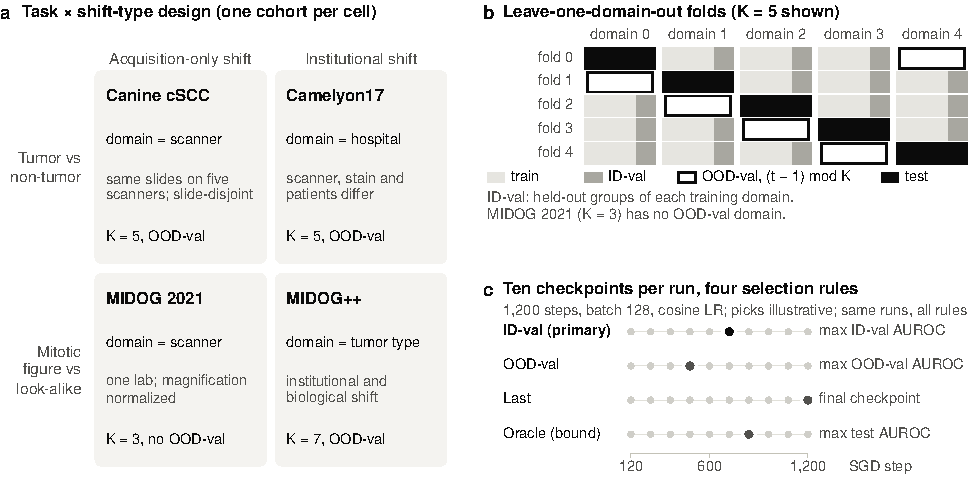
\includegraphics[width=\linewidth]{fig_design}
  \caption{Study design. (a) The four cohorts cross the task with the type of
  shift, one cohort per cell. (b) Leave-one-domain-out folds for $K=5$: fold $t$
  tests domain $t$, validates out of distribution on domain $(t-1)\bmod K$ and
  holds out ID-validation groups of every training domain. (c) Every run is
  checkpointed ten times and evaluated under four selection rules; the
  positions of the selected checkpoints are illustrative.}
  \label{fig:design}
\end{figure}

\begin{table}[width=\linewidth,pos=t]
\caption{Cohorts and per-fold split sizes (number of patches; a range is
the minimum--maximum over folds). Counts are identical at 64 and 96~px. ID-val:
group-disjoint validation split of the training domains; OOD-val: held-out
validation domain $(t-1)\bmod K$. The un-normalized MIDOG~2021 variant, used as
a compact-tier sensitivity analysis, has the same split sizes as MIDOG~2021.}
\label{tab:cohorts}
\footnotesize
\begin{tabular*}{\tblwidth}{@{\extracolsep{\fill}}>{\raggedright\arraybackslash}p{2.5cm}*{4}{>{\raggedright\arraybackslash}p{3.05cm}}@{}}
\toprule
 & Camelyon17-WILDS & Canine cSCC & MIDOG 2021 & MIDOG++ \\
\midrule
Task (pos.\ vs neg.) & tumor vs normal (lymph node) & SCC tumor vs non-tumor tissue
  & mitotic figure vs look-alike & mitotic figure vs look-alike \\
Domain & hospital & scanner (same 44 slides) & scanner (one lab) & tumor type \\
$K$ & 5 & 5 & 3 & 7 \\
Shift type & institutional & acquisition-only & acquisition-only
  & institutional and biological \\
Disjoint group & patient & slide & image & image \\
OOD-val domain & yes & yes & none & yes \\
Scale normalization & none (native patch) & per scanner, to CS2 & 0.25\,\textmu m/px & 0.25\,\textmu m/px \\
\midrule
Train & 30,000 & 22,872--26,596 & 2,160--2,544 & 11,854--17,940 \\
ID-val & 12,000 & 3,895--4,780 & 597--716 & 2,555--3,891 \\
OOD-val & 12,000 & 2,197--3,745 & -- & 1,806--8,216 \\
Test & 25,000 & 2,197--3,745 & 1,175--1,648 & 1,806--8,216 \\
Unlabeled pool & 40,000 & 40,000 & 25,200 & 40,000 \\
Positive rate, train & 0.50 & 0.52--0.55 & 0.35--0.39 & 0.42--0.49 \\
Positive rate, test & 0.50 & 0.51--0.59 & 0.35--0.43 & 0.27--0.63 \\
\bottomrule
\end{tabular*}
\end{table}

\paragraph{Cohort construction} Camelyon17-WILDS provides $96\times96$~px
lymph-node patches from five hospitals \citep{koh2021wilds,bandi2019camelyon17};
ID validation holds out whole patients of every training hospital. In the
canine cohort, each of 44 slides was digitized with five scanners
\citep{wilm2023canine}. The slides are split into five groups, so that a test
domain is a new scanner and a set of slides that is absent from training under
every scanner, and magnification is normalized to the CS2 scanner. MIDOG~2021
\citep{aubreville2023midog} has 150 annotated breast cancer images from one
laboratory, 50 per scanner. The scanners' resolutions differ by about 11\%, so
the primary cache normalizes every image to 0.25~\textmu m/px; the
un-normalized cache is a compact-tier sensitivity analysis. MIDOG++
\citep{aubreville2023midogpp} provides 503 images of seven tumor types from two
species, and its 150 breast cancer images are the MIDOG~2021 images. Mitosis
patches are centered on annotated mitotic figures and non-mitotic look-alikes.
The unlabeled pools used for self-supervision come only from the training
domains and exclude all validation and test groups, so the self-supervised arms
remain domain generalization methods. Sampling, scale normalization, the
MIDOG++ domains and the handling of objects near image borders are detailed in
Supplementary Section~\ref{S-sup:setup}.

\subsection{Model tiers}
\label{sec:setup-models}

\paragraph{Compact tier (C)} The compact model is a four-stage convolutional
network on 64~px input with 583,394 parameters. Stages 1--3 each apply two
$3\times3$ convolution--batch normalization--ReLU blocks followed by $2\times2$
max pooling, with 32, 64 and 128 channels. Stage 4 is one such block with 256
channels, followed by global average pooling and a linear layer with two
outputs. It is trained from random initialization, and inputs are normalized
with ImageNet channel statistics.

\paragraph{Standard tier (S)} ResNet-50 \citep{he2016resnet} with ImageNet
initialization \citep{deng2009imagenet} is fine-tuned end to end at the native
96~px. Two pathology foundation models of \citet{kang2023benchmarking} are also
used: a Barlow Twins ResNet-50, fine-tuned at 96~px, and a DINO ViT-S/16
\citep{dosovitskiy2021vit}, fine-tuned on inputs upsampled bilinearly to
224~px. Their inputs are normalized with the channel statistics released with
the weights. Frozen linear probes on ImageNet ResNet-50, Barlow Twins ResNet-50
and DINO ViT-S/16 follow one rule: the input is upsampled to 224~px, and
features are extracted in fp32 and standardized with the training-split mean
and SD. A linear head is trained with SGD (learning rate 0.05, momentum 0.9,
weight decay $10^{-4}$, 1,200 steps of 128) and selected like every other arm.
A supplementary representation ladder applies the same probe to nine frozen
backbones. \citet{kang2023benchmarking} pre-trained on 19 million patches from
20,994 TCGA whole-slide images, and the released checkpoints are these
TCGA-only models. None of our cohorts comes from TCGA. Camelyon17 comes
from Dutch hospitals, the canine slides from the veterinary CATCH collection
\citep{wilm2023canine}, and
MIDOG++ from veterinary laboratories and UMC Utrecht. The pre-training images
therefore do not overlap with ours, although some organs (breast, skin) occur in
both.

\subsection{Optimization and checkpointing}
\label{sec:setup-optim}

Training uses the fixed budget of Section~\ref{sec:protocol-lodo}: batches of
128 drawn without replacement and reshuffled every epoch, and a cosine schedule.
The compact tier uses SGD (momentum 0.9, weight decay $10^{-4}$) with a fixed,
untuned learning rate of 0.02. The standard-tier ResNet-50 arms use SGD with
the same momentum and weight decay. Their learning rate is selected per fold
from $\{10^{-3},3\times10^{-3},10^{-2},3\times10^{-2},10^{-1}\}$ on ImageNet
ERM and shared by every ImageNet ResNet-50 arm of the fold. The grid was extended
upward twice because the selected rate sat on its upper edge. The Barlow Twins
fine-tunes have their own per-fold rate, selected on Barlow Twins ERM from
$\{3\times10^{-4},10^{-3},3\times10^{-3},10^{-2},3\times10^{-2}\}$. Inheriting
the ImageNet rate made their training fail on some folds
(Supplementary Section~\ref{S-app:tuning}). The ViT uses
AdamW (weight decay 0.05, 5\% linear warm-up) with a learning rate selected per
fold from $\{10^{-5},3\times10^{-5},10^{-4}\}$. Every arm except the frozen
probes receives a random dihedral augmentation (flips and rotations by
multiples of $90^\circ$, drawn per batch). The standard tier trains in
bfloat16 autocast and the compact tier in fp32. Evaluation is always in fp32,
with float64 probabilities. TF32 is enabled, and kernels are not forced to be
deterministic. At each checkpoint the record stores eight metrics per split
(AUROC, average precision, accuracy, balanced accuracy, F1, ECE, Brier score,
negative log-likelihood) and the ID-validation AUROC of each training domain.
Predictions at the selected checkpoints and the ID-selected weights are also
saved. A run whose loss or predictions become non-finite is stopped, marked as
diverged and kept in the analysis, with non-finite probabilities scored as 0.5.
Six of the 3,400 final runs diverged, all IRM: two at the compact tier and
four at the standard tier. Camelyon17 models are also scored on the
PatchCamelyon test split \citep{veeling2018pcam}, center-cropped to 64~px at the
compact tier. This score is never used for selection.

\subsection{Arms}
\label{sec:setup-arms}

Table~\ref{tab:arms} lists every arm with its implementation and grid. Arms
that combine two components inherit the tuned value of their parent:
SimCLR+SAM takes $\rho$ from SAM, and the foundation-model H\&E-jitter arms
take $s$ from standard-tier H\&E jitter.

\begin{table}[width=\linewidth,pos=p]
\caption{Arms, implementations and hyperparameter grids. Grids are searched
per fold with seed~0 and selected by ID-validation AUROC; values outside a
grid are fixed. Tier: C = compact CNN (64~px), S = standard (96~px). All
fine-tuned arms also receive the shared dihedral augmentation. $^{\dagger}$Transductive: uses the unlabeled images of the test domain.}
\label{tab:arms}
\footnotesize
\begin{tabular*}{\tblwidth}{@{\extracolsep{\fill}}>{\raggedright\arraybackslash}p{2.4cm}>{\raggedright\arraybackslash}p{7.4cm}>{\raggedright\arraybackslash}p{4.4cm}l@{}}
\toprule
Arm & Implementation & Grid / fixed values & Tier \\
\midrule
\multicolumn{4}{@{}l}{\emph{Baseline and controls}}\\
ERM & Cross-entropy. & C: lr 0.02; S: lr $\in\{10^{-3},3{\times}10^{-3},\dots,10^{-1}\}$ & C, S \\
Augmentation-only & SimCLR's view augmentation (random resized crop, flips, rotations, color jitter, grayscale) applied to supervised batches; no contrastive loss. & crop scale $[0.4,1]$; jitter 0.4 with prob.\ 0.8; hue offset 0.08; grayscale prob.\ 0.2 & C \\
Compute-matched ERM & ERM for $1{,}200+\lceil I_{\text{SSL}}/128\rceil$ steps; $I_{\text{SSL}}$ = images passed through the encoder during SimCLR pre-training (two views per image). & 4,944 steps ($|U|=40{,}000$); 3,552 steps (MIDOG~2021, $|U|=25{,}200$) & C \\
\midrule
\multicolumn{4}{@{}l}{\emph{Optimization and self-supervision}}\\
SAM \citep{foret2021sam} & SGD base optimizer; batch-norm statistics updated on the unperturbed pass only. & $\rho\in\{0.02,0.05,0.1\}$ & C, S \\
SimCLR \citep{chen2020simclr} & NT-Xent pre-training on the fold's unlabeled pool (C: from scratch; S: continued from ImageNet), 2-layer projection head, then ERM fine-tuning. & $\tau=0.5$, batch 256, 6 epochs, lr 0.05 (C) / 0.01 (S) & C, S \\
SimCLR+SAM & SimCLR initialization, SAM fine-tuning. & $\rho$ from SAM & C \\
\midrule
\multicolumn{4}{@{}l}{\emph{Domain-aware training (uses training-domain labels)}}\\
GroupDRO \citep{sagawa2020groupdro} & Weights over training domains, $q_k\leftarrow q_k e^{\eta L_k}$, loss $\sum_k q_kL_k$; domains absent from a batch are not updated. & $\eta\in\{10^{-3},10^{-2},10^{-1}\}$ & C, S \\
IRMv1 \citep{arjovsky2019irm} & Split-batch penalty per domain, averaged over domains; weight 1 for the first 25\% of steps, then $\lambda$, with optimizer reset. & $\lambda\in\{1,10,100\}$ & C, S \\
DeepCORAL \citep{sun2016coral} & Squared differences of feature means and covariances, averaged over pairs of training domains. & $\lambda\in\{0.1,1,10\}$ & C, S \\
MixStyle \citep{zhou2021mixstyle} & Random mixing of instance feature statistics after stages 1 and 2 (C) or ResNet layers 1 and 2 (S); identity at evaluation. & $p\in\{0.5,1\}\times\alpha\in\{0.1,0.3\}$ & C, S \\
Fish \citep{shi2022fish} & Inner copy takes one SGD step per training domain in the batch (random order, persistent inner optimizer); $\theta\leftarrow\theta+\epsilon(\tilde\theta-\theta)$ for parameters, batch-norm buffers copied. & $\epsilon\in\{0.01,0.05,0.1,0.5\}$ & C, S \\
LISA \citep{yao2022lisa} & Per batch, intra-label mixup across domains (prob.\ $p_{\text{sel}}$) or intra-domain mixup across labels; $\lambda\sim\mathrm{Beta}(\alpha,\alpha)$, soft labels. & $\alpha\in\{0.5,2\}\times p_{\text{sel}}\in\{0.5,1\}$ & C, S \\
\midrule
\multicolumn{4}{@{}l}{\emph{Stain normalization and color augmentation}}\\
Macenko$^{\dagger}$ \citep{macenko2009} & One stain estimate per slide and scanner, mapped to a reference fitted with the same estimator on the training slides; every split. & $I_0=240$, OD threshold 0.15, angle percentile 1; $\le$256 tiles per slide & C, S \\
H\&E jitter & Per-image brightness, contrast and saturation factors $\sim U[1-s,1+s]$ and per-channel offsets $\sim U[-s/5,s/5]$. & $s\in\{0.2,0.4\}$ & C, S \\
TIA-style$^{\dagger}$ & Per-slide Macenko normalization followed by H\&E jitter. & $s=0.3$ & C, S \\
Per-tile Macenko & One stain estimate per tile (Supplementary Section~\ref{S-app:macenko}). & as Macenko & C, S \\
\midrule
\multicolumn{4}{@{}l}{\emph{Test-time adaptation (on the ID-selected checkpoint)}}\\
BN-adapt$^{\dagger}$ \citep{schneider2020bn} & Batch-norm statistics re-estimated (cumulative average) on the shuffled test stream in batches of 128, then prediction. & on ERM, SimCLR, H\&E jitter (C); ERM (S) & C, S \\
TENT$^{\dagger}$ \citep{wang2021tent} & Online entropy minimization of batch-norm affine parameters (Adam, lr $10^{-3}$, one step per batch of 128, shuffled stream); a batch is predicted before its update. & on ERM & C \\
\midrule
\multicolumn{4}{@{}l}{\emph{Pathology foundation models \citep{kang2023benchmarking}}}\\
Barlow Twins RN50: ERM, +H\&E jitter & Fine-tuned at 96~px. & lr $\in\{3{\times}10^{-4},\dots,3{\times}10^{-2}\}$ on BT ERM; $s$ from H\&E jitter & S \\
DINO ViT-S/16: ERM, +H\&E jitter & Fine-tuned at 224~px, AdamW. & lr $\in\{10^{-5},3{\times}10^{-5},10^{-4}\}$; $s$ from H\&E jitter & S \\
Frozen probes & Linear head on frozen ImageNet RN50, Barlow Twins RN50 or DINO ViT-S/16 features at 224~px. & lr 0.05 & S \\
\bottomrule
\end{tabular*}
\end{table}

\paragraph{Controls for self-supervision} The augmentation-only control
applies SimCLR's view augmentation to labeled batches without the contrastive
loss, which separates the effect of the augmentations from that of
pre-training. The compute-matched control gives ERM as many images through the
encoder as SimCLR receives in pre-training and fine-tuning together
(Table~\ref{tab:arms}).

\paragraph{Stain normalization} As in common practice, Macenko's stain matrix
\citep{macenko2009} is estimated once per slide imaged on one scanner, from the
pooled tissue pixels of up to 256 of its tiles, with concentrations clamped at
zero, and is mapped to a reference fitted with the same estimator on the
training slides. No labels are used, but the method is transductive: each test
slide is normalized from its own tiles. The per-tile variant estimates the
stain matrix on every tile separately. Implementation details are in
Supplementary Section~\ref{S-sup:setup}, and the effect of the granularity in
Supplementary Section~\ref{S-app:macenko}. Our H\&E jitter perturbs RGB color; it
is not an augmentation in HED space.

\paragraph{Test-time adaptation} BN-adapt and TENT process the test split in a
seed-specific random order. Each batch of 128 therefore contains both classes
in roughly the test domain's proportion. A label-sorted stream would give
single-class batches and an uninformative adapted AUROC.

\paragraph{Transductive arms} BN-adapt, TENT, Macenko and TIA-style use the
unlabeled images of the test domain at prediction time; the other arms see one
test image at a time. The four transductive arms are marked in every table and
figure and are not directly comparable with the inductive arms.

\paragraph{Dropped arm} The rotation-invariance arm of the previous version was
dropped. In this pipeline it reduced to the dihedral augmentation that every arm
receives, so it was identical to ERM.

\subsection{Seeds, compute and availability}
\label{sec:setup-compute}

Final runs use seeds 0--4 at the compact tier and 0--2 at the standard tier.
Tuning uses seed~0 and is stored separately from the final runs. The planned
design has the following runs:
\begin{itemize}
  \item tuning: 520 at the compact tier (26 configurations, 20 folds) plus 78
    for the un-normalized MIDOG~2021 cohort; at the standard tier, 160
    learning-rate runs (100 ResNet-50, 60 ViT), 100 Barlow Twins
    learning-rate runs and 520 method-grid runs;
  \item final: 1,600 at the compact tier (16 arms, 5 seeds, 20 folds), 240 for
    the un-normalized MIDOG~2021 sensitivity analysis, and 1,200 at the standard
    tier (20 arms, 3 seeds, 20 folds);
  \item representation ladder: 360 runs.
\end{itemize}
Test-time adaptation is evaluated within the run of the base arm. All 4,778 runs
(1,378 tuning and 3,400 final, the ladder included) completed. They ran on
NVIDIA H100 NVL GPUs and used about 34 GPU-hours, not counting development
and diagnostic runs. Each
record contains the full hyperparameters, a SHA-256 hash of the training code
and a fingerprint of the fold cache. A record whose fingerprint or
hyperparameters do not match the job is recomputed. Code, fold-construction
scripts, all run records and the scripts that regenerate every table and figure
are available at \coderepo\ \TBD{Zenodo DOI of the archived release}.

%% Results (MedIA revision, v2 pipeline).
%% Every number is read from results/v2/analysis/{C,S}/... (snapshot 1381bdd759f9; ID-validation
%% selection unless stated), from the tables generated by src/v2/paper_tables.py (paper/media/tables/)
%% or from results/v2/analysis/paper_numbers.json, which the same script writes.
\section{Results}
\label{sec:results}

No model is trained on labeled data from its test domain. Apart from the
test-time adaptation arms, which use unlabeled test images, every result below
is the performance of a model applied unchanged to an unseen site.
Unless stated otherwise, results use the primary model-selection rule
(training-domain validation) and test AUROC. We lead with the standard tier,
whose models are closer to current practice, and give the compact tier
alongside. Arms marked $^{\dagger}$ use unlabeled test-domain images and are
not like-for-like competitors of the other arms
(Section~\ref{sec:setup-arms}).

\subsection{Performance at every held-out domain}
\label{sec:results-domains}

Figure~\ref{fig:perdomain} shows the seed-mean test AUROC of every
standard-tier arm at every held-out domain, and Table~\ref{tab:main-S}
summarizes it by the worst domain and the mean. Averages hide large
differences between domains. Standard-tier ERM has a mean AUROC of 0.785 on
the canine cohort but scores 0.534 on the 3DHistech P1000 scanner, which is
close to chance. That scanner is the worst domain for 17 of the 21 arms. On
Camelyon17, ERM averages 0.955 and drops to 0.895 at center~2. The two mitosis
cohorts are flatter: ERM ranges from 0.847 to 0.879 on MIDOG~2021 and from
0.870 to 0.927 on MIDOG++. The compact tier shows the same pattern at a lower
level (Supplementary Table~\ref{S-tab:main-C}). There, ERM's worst domains score
0.698 (Camelyon17), 0.551 (canine), 0.765 (MIDOG~2021) and 0.766 (MIDOG++).

The worst domain is not the same for every arm. On Camelyon17, center~2 is the
worst domain for 10 of 21 standard-tier arms, and the others fail at
centers~1, 3 or 4. A study that reports a single held-out hospital therefore
measures one point of a distribution whose shape depends on the method.

\begin{figure}[pos=tbp]
  \centering
  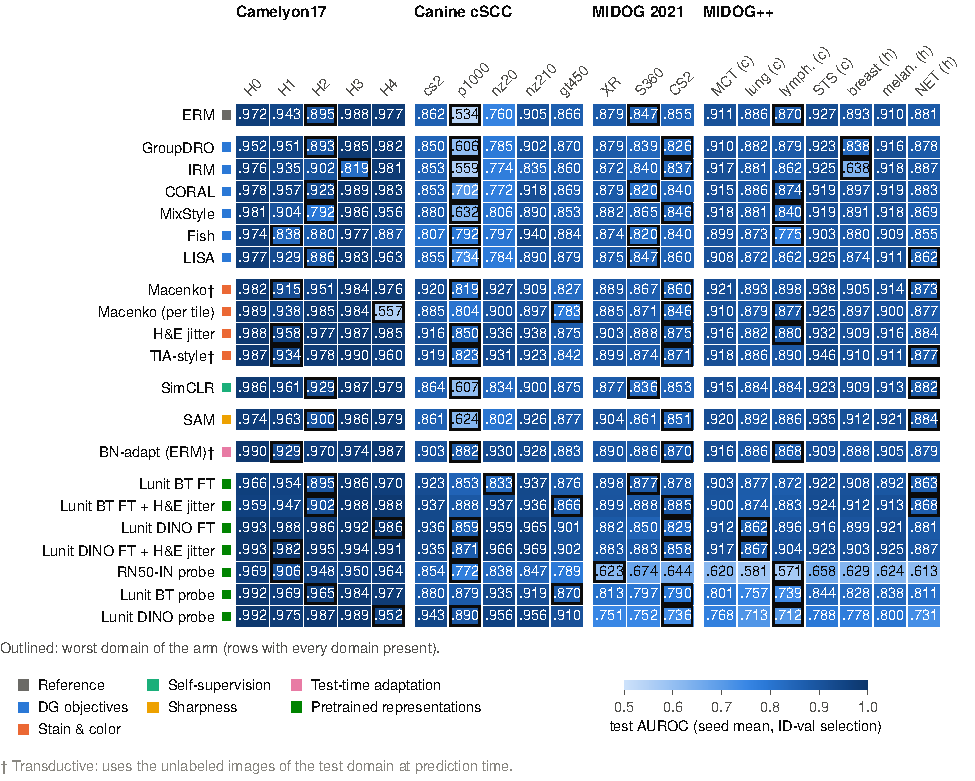
\includegraphics[width=\linewidth]{fig_perdomain_S}
  \caption{Test AUROC of every standard-tier arm at every held-out domain
  (mean over three seeds; ID-validation selection). Outlined cells mark each
  arm's worst domain. Domains: Camelyon17 hospitals H0--H4; canine scanners;
  MIDOG~2021 scanners; MIDOG++ tumor types ((c) canine, (h) human).
  $^{\dagger}$Transductive: uses the unlabeled images of the test domain at
  prediction time. The compact tier is in Supplementary
  Fig.~\ref{S-fig:perdomain-C}.}
  \label{fig:perdomain}
\end{figure}

\begin{table}[width=\linewidth,pos=p]
\caption{Standard tier: worst-domain AUROC (rank among the 21 arms) and mean
AUROC over held-out domains, ID-validation selection, three seeds. Bold: best
worst-domain AUROC in the cohort. $^{\dagger}$Transductive. FT: fine-tuned;
BT: Barlow Twins; IN: ImageNet. The compact tier is in Supplementary
Table~\ref{S-tab:main-C}.}
\label{tab:main-S}
\footnotesize
\setlength{\tabcolsep}{3pt}
% generated by src/v2/paper_tables.py from results/v2/analysis/S/*/summary_id.csv, ranks_id.csv
\begin{tabular*}{\tblwidth}{@{\extracolsep{\fill}}l*{4}{rr}@{}}
\toprule
Arm & \multicolumn{2}{c}{Camelyon17 ($K=5$)} & \multicolumn{2}{c}{Canine cSCC ($K=5$)} & \multicolumn{2}{c}{MIDOG 2021 ($K=3$)} & \multicolumn{2}{c}{MIDOG++ ($K=7$)} \\
\cmidrule(lr){2-3}\cmidrule(lr){4-5}\cmidrule(lr){6-7}\cmidrule(lr){8-9}
 & worst (rank) & mean & worst (rank) & mean & worst (rank) & mean & worst (rank) & mean \\
\midrule
\multicolumn{9}{@{}l}{\emph{Reference and controls}}\\
ERM & 0.895 (14) & 0.955 & 0.534 (21) & 0.785 & 0.847 (10) & 0.860 & 0.870 (8) & 0.897 \\
\addlinespace[2pt]
\multicolumn{9}{@{}l}{\emph{Domain-aware training}}\\
GroupDRO & 0.893 (16) & 0.953 & 0.606 (19) & 0.803 & 0.826 (16) & 0.848 & 0.838 (16) & 0.890 \\
IRM & 0.819 (19) & 0.923 & 0.559 (20) & 0.776 & 0.837 (13) & 0.850 & 0.638 (20) & 0.861 \\
CORAL & 0.923 (9) & 0.966 & 0.702 (15) & 0.823 & 0.820 (18) & 0.846 & 0.874 (6) & 0.899 \\
MixStyle & 0.792 (20) & 0.924 & 0.632 (16) & 0.812 & 0.846 (11) & 0.864 & 0.840 (15) & 0.891 \\
Fish & 0.838 (18) & 0.911 & 0.792 (11) & 0.844 & 0.820 (17) & 0.845 & 0.775 (17) & 0.871 \\
LISA & 0.886 (17) & 0.948 & 0.734 (14) & 0.828 & 0.847 (9) & 0.861 & 0.862 (14) & 0.888 \\
\addlinespace[2pt]
\multicolumn{9}{@{}l}{\emph{Stain normalization and color}}\\
Macenko$^{\dagger}$ & 0.915 (10) & 0.962 & 0.819 (10) & 0.881 & 0.860 (6) & 0.872 & 0.873 (7) & 0.906 \\
Macenko (per tile) & 0.557 (21) & 0.891 & 0.783 (12) & 0.854 & 0.846 (12) & 0.867 & 0.877 (5) & 0.895 \\
H\&E jitter & 0.958 (4) & 0.979 & 0.850 (7) & 0.903 & 0.875 (3) & 0.888 & 0.880 (3) & 0.903 \\
TIA-style$^{\dagger}$ & 0.934 (6) & 0.970 & 0.823 (9) & 0.887 & 0.871 (4) & 0.881 & 0.877 (4) & 0.905 \\
\addlinespace[2pt]
\multicolumn{9}{@{}l}{\emph{Self-supervision}}\\
SimCLR & 0.929 (7) & 0.968 & 0.607 (18) & 0.816 & 0.836 (14) & 0.855 & 0.882 (2) & 0.901 \\
\addlinespace[2pt]
\multicolumn{9}{@{}l}{\emph{Sharpness-aware}}\\
SAM & 0.900 (13) & 0.960 & 0.624 (17) & 0.818 & 0.851 (8) & 0.872 & \textbf{0.884} (1) & 0.907 \\
\addlinespace[2pt]
\multicolumn{9}{@{}l}{\emph{Test-time adaptation}}\\
BN-adapt (ERM)$^{\dagger}$ & 0.929 (8) & 0.970 & 0.882 (2) & 0.905 & 0.870 (5) & 0.882 & 0.868 (9) & 0.893 \\
\addlinespace[2pt]
\multicolumn{9}{@{}l}{\emph{Pretrained representations}}\\
Lunit BT FT & 0.895 (15) & 0.954 & 0.833 (8) & 0.885 & 0.877 (2) & 0.885 & 0.863 (12) & 0.891 \\
Lunit BT FT + H\&E jitter & 0.902 (12) & 0.957 & 0.866 (5) & 0.913 & \textbf{0.885} (1) & 0.891 & 0.868 (10) & 0.896 \\
Lunit DINO FT & \textbf{0.986} (1) & 0.989 & 0.859 (6) & 0.924 & 0.829 (15) & 0.854 & 0.862 (13) & 0.898 \\
Lunit DINO FT + H\&E jitter & 0.982 (2) & 0.991 & 0.871 (3) & 0.929 & 0.858 (7) & 0.875 & 0.867 (11) & 0.904 \\
RN50-IN probe & 0.906 (11) & 0.948 & 0.772 (13) & 0.820 & 0.623 (21) & 0.647 & 0.571 (21) & 0.614 \\
Lunit BT probe & 0.965 (3) & 0.977 & 0.870 (4) & 0.896 & 0.790 (19) & 0.800 & 0.739 (18) & 0.802 \\
Lunit DINO probe & 0.952 (5) & 0.979 & \textbf{0.890} (1) & 0.931 & 0.736 (20) & 0.746 & 0.712 (19) & 0.756 \\
\bottomrule
\end{tabular*}

\end{table}

\subsection{Where the variance of a held-out score comes from}
\label{sec:results-variance}

Figure~\ref{fig:variance} and Table~\ref{tab:evidence} report the variance
decomposition of Section~\ref{sec:protocol-variance}. For most arms, most of
the variance of a single run is due to which domain is held out. The median
ICC over arms lies between 0.72 and 0.95 in every cohort and at both tiers.
It is highest on the canine cohort and MIDOG++ at the standard tier (0.95 in
both), where 20 of 21 and 18 of 21 arms have an ICC interval whose lower limit
exceeds 0.5. For comparison, the same estimators give a median ICC of 0.98 on
DomainBed's published results outside TerraIncognita
(Supplementary Section~\ref{S-app:domainbed}).

Run-to-run noise is nevertheless far from negligible, and it is largest at
the hard domains. At the compact tier, the five ERM seeds at Camelyon17
center~2 span 0.599 to 0.929 AUROC, and at center~4, ERM's worst domain, they
span 0.592 to 0.797 (Supplementary Fig.~\ref{S-fig:seedspread}). At the standard
tier, the three ERM seeds on the canine P1000 scanner span 0.461 to 0.598. For
some arms the spread at the worst domain is larger still: the seeds of
standard-tier IRM at Camelyon17 center~3 span 0.50 to 0.98, and those of
compact-tier per-tile Macenko at center~4 span 0.41 to 0.74.

The intervals are wide. On MIDOG~2021, with $K=3$, only 3 of 21 standard-tier
arms have an ICC lower limit above 0.5, and for five arms the lower limit is
zero. Estimates at the zero boundary occur for three standard-tier arms on
Camelyon17, and the Bayesian posterior gives them one-sided intervals
(Fig.~\ref{fig:variance}a). The ICC is therefore best read as a coarse
description of each cohort, not as a property of a method.

\begin{figure}[pos=tbp]
  \centering
  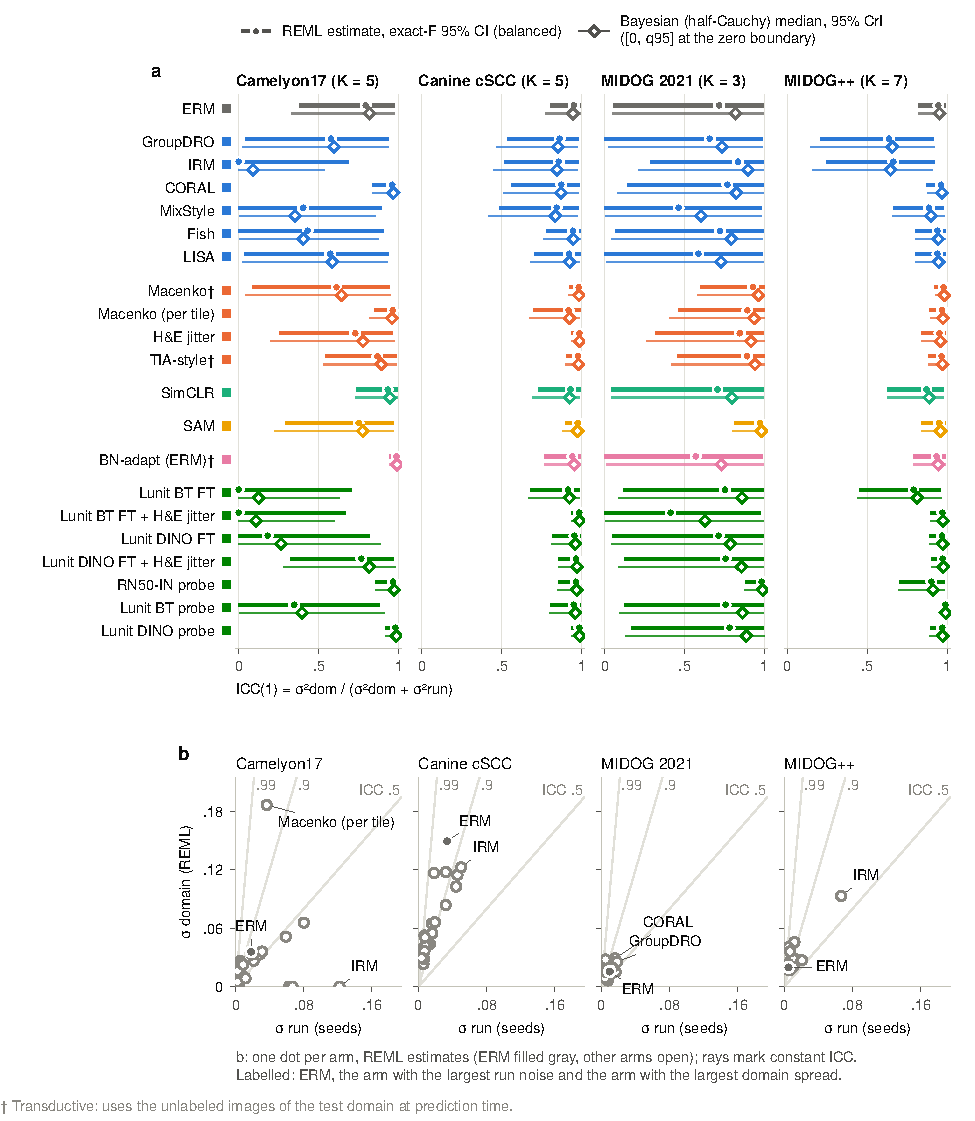
\includegraphics[width=0.92\linewidth]{fig_variance_S}
  \caption{Variance decomposition at the standard tier. (a) ICC(1), the share
  of single-run variance due to the held-out domain, with the REML estimate and
  exact-$F$ 95\% interval and the Bayesian (half-Cauchy) posterior median and
  95\% credible interval; one-sided $[0,q_{0.95}]$ at the zero boundary.
  (b) Between-domain SD $\hat\sigma_D$ against between-run SD $\hat\sigma_R$
  per arm; rays mark constant ICC. $^{\dagger}$Transductive. The compact tier
  is in Supplementary Fig.~\ref{S-fig:variance-C}.}
  \label{fig:variance}
\end{figure}

\begin{table}[width=\linewidth,pos=t]
\caption{Summary of the evidence per tier and cohort (ID-validation selection).
ICC: median and interquartile range over arms, and the number of arms whose
exact 95\% ICC interval has a lower limit above 0.5. ERM
$\hat\sigma_D$/$\hat\sigma_R$: between-domain and between-run SD of ERM.
$p<0.05$ and Holm: number of arms whose paired mean difference from ERM is
significant before and after Holm adjustment, split into better ($+$) and worse
($-$). Largest mean gain: the arm with the largest mean AUROC difference from
ERM. $\hat\sigma_\Delta$: median over arms of the SD of the per-domain
difference from ERM with the tier's seed count (Eq.~\ref{eq:diffvar}).
$K_{0.05}$: median over arms of the number of domains needed for 80\% power to
detect a mean gain of 0.05 AUROC, for independent folds and, in brackets, under
fold dependence $\rho=0.5$ (Eq.~\ref{eq:power}). Seeds: 3 (S), 5 (C).
$^{\dagger}$Transductive.}
\label{tab:evidence}
\footnotesize
\setlength{\tabcolsep}{2.5pt}
% generated by src/v2/paper_tables.py from variance_id.csv, contrasts_id.csv, power_id.csv
\begin{tabular*}{\tblwidth}{@{\extracolsep{\fill}}llrlrlrr>{\raggedright\arraybackslash}p{2.2cm}rr@{}}
\toprule
Tier & Cohort & $K$ & ICC median [IQR] & CI$_{\text{lo}}>0.5$ & ERM $\hat\sigma_D$ / $\hat\sigma_R$ & $p<0.05$ ($+$/$-$) & Holm ($+$/$-$) & Largest gain over ERM & $\hat\sigma_\Delta$ & $K_{0.05}$ \\
\midrule
S & C17 & 5 & 0.73 [0.40, 0.93] & 7/21 & 0.036 / 0.018 & 0 / 0 & 0 / 0 & Lunit DINO FT + H\&E jitter (+0.036) & 0.036 & 7 (14) \\
 & Canine & 5 & 0.95 [0.92, 0.98] & 20/21 & 0.149 / 0.034 & 0 / 0 & 0 / 0 & Lunit DINO probe (+0.145) & 0.126 & 53 (137) \\
 & MIDOG21 & 3 & 0.76 [0.71, 0.85] & 3/21 & 0.016 / 0.010 & 4 / 3 & 0 / 0 & Lunit BT FT + H\&E jitter (+0.031) & 0.013 & 3 (4) \\
 & MIDOG++ & 7 & 0.95 [0.90, 0.97] & 18/21 & 0.020 / 0.005 & 2 / 4 & 0 / 3 & SAM (+0.010) & 0.012 & 3 (5) \\
\addlinespace[3pt]
C & C17 & 5 & 0.81 [0.67, 0.89] & 11/20 & 0.101 / 0.080 & 0 / 1 & 0 / 0 & TIA-style$^{\dagger}$ (+0.107) & 0.094 & 30 (76) \\
 & Canine & 5 & 0.80 [0.68, 0.88] & 10/20 & 0.103 / 0.055 & 0 / 0 & 0 / 0 & BN-adapt (ERM)$^{\dagger}$ (+0.123) & 0.103 & 36 (92) \\
 & MIDOG21 & 3 & 0.72 [0.38, 0.83] & 3/20 & 0.037 / 0.025 & 7 / 0 & 0 / 0 & BN-adapt (H\&E jitter)$^{\dagger}$ (+0.091) & 0.028 & 5 (8) \\
 & MIDOG++ & 7 & 0.85 [0.79, 0.92] & 16/20 & 0.033 / 0.014 & 5 / 7 & 2 / 3 & Compute-matched ERM (+0.060) & 0.023 & 4 (10) \\
\bottomrule
\end{tabular*}

\end{table}

\subsection{Can the differences between methods be detected?}
\label{sec:results-contrasts}

Table~\ref{tab:evidence} counts the paired comparisons with ERM. At the
standard tier, no arm is significantly better than ERM after Holm adjustment in
any cohort. The only Holm-significant differences are three frozen linear
probes that are worse than ERM on MIDOG++. At the compact tier, two arms
improve on ERM after adjustment, both on MIDOG++: compute-matched ERM ($+0.060$)
and per-slide Macenko$^{\dagger}$ ($+0.041$). The augmentation-only control,
LISA and IRM are significantly worse there.

Lack of significance does not mean that the differences are small. On the
canine cohort, the Lunit DINO frozen probe improves mean AUROC over ERM by
0.145 and is better at all five scanners, yet its unadjusted $p$ is 0.071.
With five domains, even an exact sign-flip test cannot go below 0.0625 when
every domain improves. On the tumor cohorts the gains are large but vary
strongly from domain to domain. On the mitosis cohorts the reverse holds: the
differences are measured precisely but are small. The largest standard-tier
gain on MIDOG++ is $+0.010$ (SAM, better at all seven domains, Holm
$p=0.053$).

The power analysis puts numbers on this (Fig.~\ref{fig:power},
Table~\ref{tab:evidence}). The SD of the per-domain difference from ERM,
$\hat\sigma_\Delta$, has a median of 0.012--0.028 on the mitosis cohorts but
0.036--0.126 on the tumor cohorts. For a median arm to detect a mean gain of
0.05 AUROC with 80\% power, the standard tier would need 7 Camelyon17
hospitals and 53 canine scanners. The compact tier would need 30 and 36. If
the folds are correlated through their shared training domains
($\rho=0.5$), these numbers roughly double or triple. On the mitosis cohorts,
3--5 domains suffice for a gain of that size, but the observed gains there are
much smaller. Adding seeds helps little once $\sigma_\Delta$ is dominated by
the domain-by-arm interaction (Fig.~\ref{fig:power}). Domains, not seeds, are
the scarce resource.

\begin{figure}[pos=tbp]
  \centering
  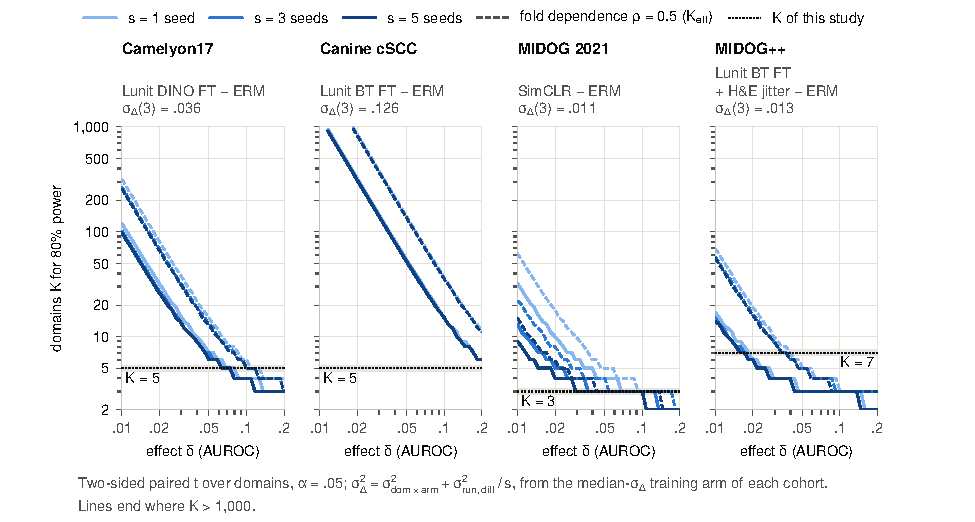
\includegraphics[width=\linewidth]{fig_power_S}
  \caption{Number of held-out domains $K$ needed for 80\% power to detect a
  mean AUROC gain $\delta$ over ERM (two-sided paired $t$ test,
  $\alpha=0.05$), at the standard tier, for the training arm with the median
  $\sigma_\Delta$ in each cohort. Solid: independent folds; dashed: fold
  dependence $\rho=0.5$; dotted: $K$ of this study. Colors: seeds per arm. The
  compact tier is in Supplementary Fig.~\ref{S-fig:power-C}.}
  \label{fig:power}
\end{figure}

\subsection{Rankings within a cohort, and the effect of model scale}
\label{sec:results-ranks}

Figure~\ref{fig:ranks}a gives each arm's worst-domain rank with bootstrap
intervals over seeds and over domains. Resampling domains usually widens the
intervals more than resampling seeds. The median width of the domain-bootstrap
interval is 3 to 7 ranks out of 21 at the standard tier, against 2 to 6 for
the seed bootstrap. Only one standard-tier arm has the rank interval $[1,1]$ under both
bootstraps: the Lunit DINO probe on the canine cohort, which ranks first in
99\% of domain resamples. The next most certain is fine-tuned Barlow Twins with
H\&E jitter on MIDOG~2021 (96\%, interval $[1,3]$). On MIDOG++, the top arm
(SAM) ranks first in only 45\% of domain resamples.

A few patterns hold across cohorts.
\begin{itemize}
  \item \emph{Pathology foundation models lead on the tumor cohorts.} The
    fine-tuned Lunit DINO ViT ranks first on Camelyon17 (worst domain 0.986),
    and its frozen probe ranks first on the canine cohort (0.890). On the
    mitosis cohorts, the frozen probes fall to the bottom: the DINO probe ranks
    20th and 19th, and the ImageNet ResNet-50 probe last on both. Fine-tuning
    narrows the gap: fine-tuned Barlow Twins with H\&E jitter ranks first on
    MIDOG~2021 (0.885), and the fine-tuned DINO ViT ranks 15th and 13th on the
    two mitosis cohorts.
  \item \emph{H\&E color jitter is consistently good.} It ranks 4th, 7th, 3rd
    and 3rd at the standard tier and 3rd, 8th, 5th and 8th at the compact
    tier.
  \item \emph{The domain-generalization objectives rarely help.} Under
    ID-validation selection, none of the six (GroupDRO, IRM, CORAL, MixStyle,
    Fish and LISA) ranks in the top five on any cohort at either tier. The
    best of them is CORAL on MIDOG++ (6th at the standard tier). Other rules
    can lift a single objective: with oracle selection, CORAL ranks 4th on
    MIDOG++ at the standard tier and LISA 2nd on the canine cohort at the
    compact tier.
  \item \emph{Transductive arms are strong.} BN-adapt on ERM ranks 2nd on the
    canine cohort, and at the compact tier BN-adapt on H\&E jitter ranks among
    the top six everywhere. Both use unlabeled test-domain images.
\end{itemize}

Model scale changes the picture (Fig.~\ref{fig:scale}). Moving from the
compact CNN to ImageNet ResNet-50 raises ERM's worst-domain AUROC on
Camelyon17 (0.698 to 0.895) and on the mitosis cohorts (0.765 to 0.847;
0.766 to 0.870), but not on the canine cohort (0.551 to 0.534). For the 14
arms run at both tiers, Kendall's $\tau_b$ between the two tiers' worst-domain
rankings is 0.60 (Camelyon17), 0.63 (canine), 0.32 (MIDOG~2021) and 0.30
(MIDOG++). Conclusions drawn from the compact model therefore transfer only in
part. Compute-matched ERM, the best compact arm on MIDOG++, was not run at the
standard tier, so that result cannot be checked there.

Hyperparameters matter as much as methods. The Barlow Twins fine-tunes first
inherited the learning rate tuned for ImageNet ResNet-50, and training failed
on some folds. Tuning their own rate raised mean off-site AUROC on MIDOG++
from 0.715 to 0.891 (Supplementary Section~\ref{S-app:tuning-bt}). Stain normalization shows
the same sensitivity to implementation. Estimating the Macenko stain matrix
per tile instead of per slide drops the arm from rank~10 to last on
Camelyon17 at the standard tier, because it fails at one center
(0.557 against 0.976 for the per-slide estimate;
Supplementary Section~\ref{S-app:macenko}).

\begin{figure}[pos=tbp]
  \centering
  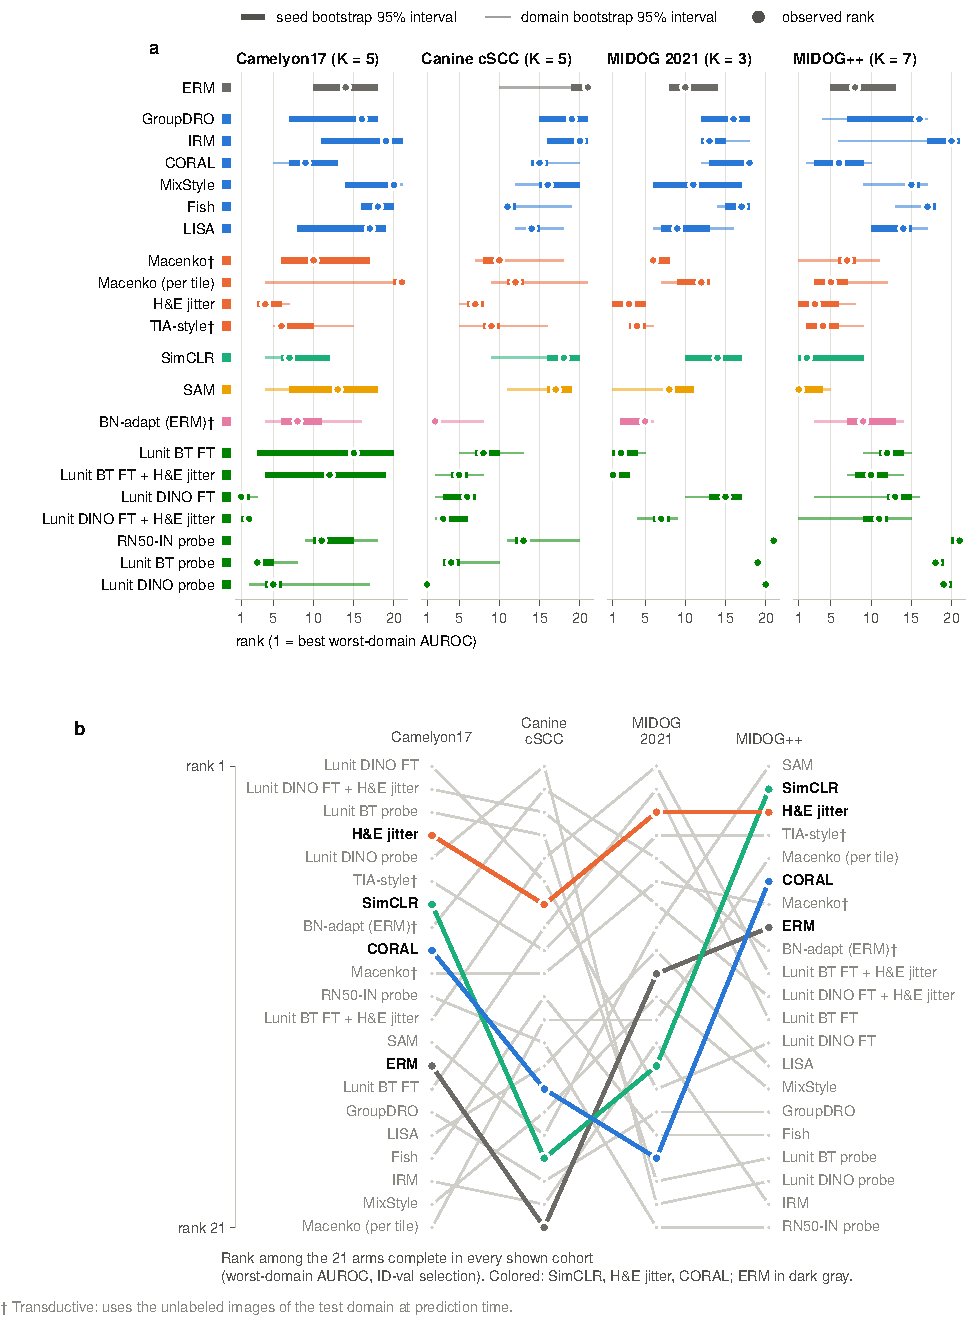
\includegraphics[width=0.85\linewidth]{fig_ranks_S}
  \caption{Rankings at the standard tier. (a) Rank by worst-domain AUROC
  (1 = best) with 95\% intervals from bootstrapping seeds within domains
  (thick) and domains (thin). (b) Ranks of all 21 arms across the four cohorts;
  ERM, SimCLR, H\&E jitter and CORAL are highlighted. $^{\dagger}$Transductive.
  The compact tier is in Supplementary Fig.~\ref{S-fig:ranks-C}.}
  \label{fig:ranks}
\end{figure}

\begin{figure}[pos=tbp]
  \centering
  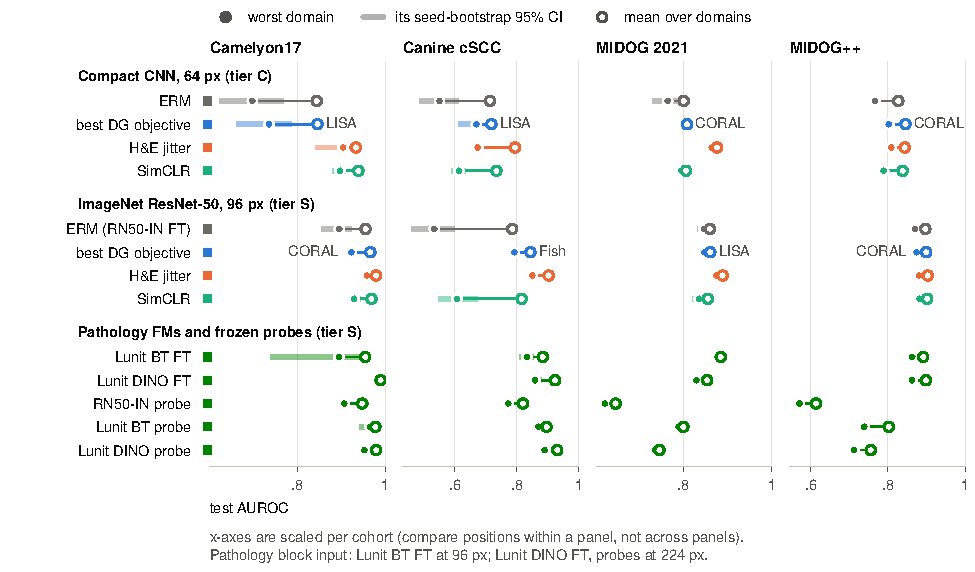
\includegraphics[width=\linewidth]{fig_scale}
  \caption{Effect of model scale and pre-training. Worst-domain AUROC (filled,
  with seed-bootstrap 95\% interval) and mean AUROC (open) for ERM, the best
  domain-generalization objective, H\&E jitter and SimCLR at the compact tier
  (compact CNN, 64~px) and the standard tier (ImageNet ResNet-50, 96~px), and
  for the pathology foundation models. The $x$-axes are scaled per cohort.}
  \label{fig:scale}
\end{figure}

\subsection{Do rankings follow the task or the type of shift?}
\label{sec:results-cross}

The arm-by-cohort interaction is significant at both tiers (wild bootstrap,
$p<0.001$ at the standard tier and $p=0.004$ at the compact tier): methods do
not rank the same way on every cohort. Figure~\ref{fig:kendall} shows how the
rankings agree between pairs of cohorts.

At the standard tier, agreement follows the task. The two tumor cohorts agree
with $\tau_b=0.43$ (95\% interval [0.28, 0.52]) and the two mitosis cohorts
with $\tau_b=0.42$ [0.30, 0.50]. The pairs that share only the shift type agree
much less (0.15 and 0.14), and the pairs that share neither do not agree at all
(0.03 and $-0.06$). The mean $\tau_b$ of same-task pairs exceeds that of
same-shift pairs by 0.28 [0.19, 0.40]. In the $2\times2$ decomposition of
Eq.~\eqref{eq:2x2}, the task contrast accounts for 84\% of the between-cohort
sum of squares, the shift contrast for 10\% and their interaction for 7\%. The
pattern is the same under the last-checkpoint (85\% task) and oracle (90\%)
rules.

At the compact tier the picture is less clear. The task contrast accounts for
51\% and the shift contrast for 32\%, and same-task pairs agree only slightly
more than same-shift pairs (difference 0.06 [$-0.04$, 0.14]). The canine and
MIDOG~2021 cohorts, which share the shift type but not the task, agree with
$\tau_b=0.54$, almost as much as the two mitosis cohorts (0.59).

Two cautions apply. First, with four cohorts there are only three ways to
split them into two pairs, and the task split ranks first among them at both
tiers. A permutation test at the cohort level cannot go below $p=1/3$. The
decomposition describes the interaction; it cannot prove that rankings are
organized by task. Second, the 150 breast-cancer images of MIDOG++ are the
MIDOG~2021 images, so the two mitosis cohorts share one of MIDOG++'s seven
domains. This overlap may raise their agreement. The tumor cohorts share no
images, and their agreement at the standard tier is as high.

\begin{figure}[pos=tbp]
  \centering
  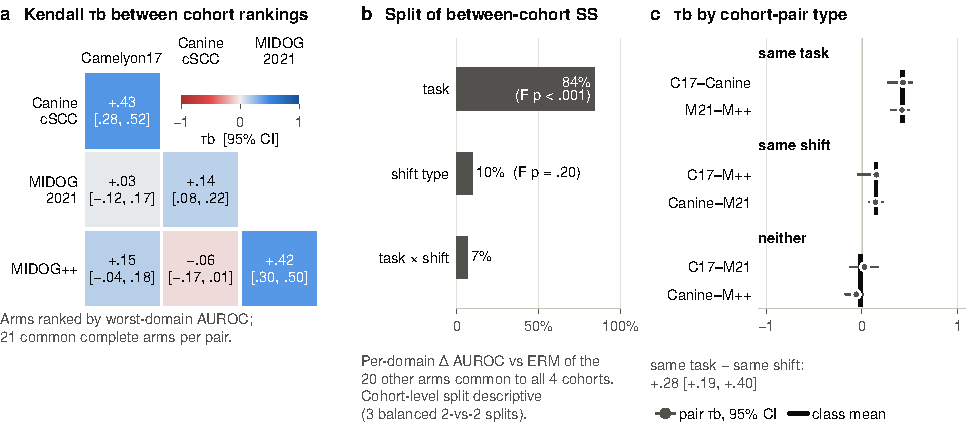
\includegraphics[width=\linewidth]{fig_kendall_S}\\[4pt]
  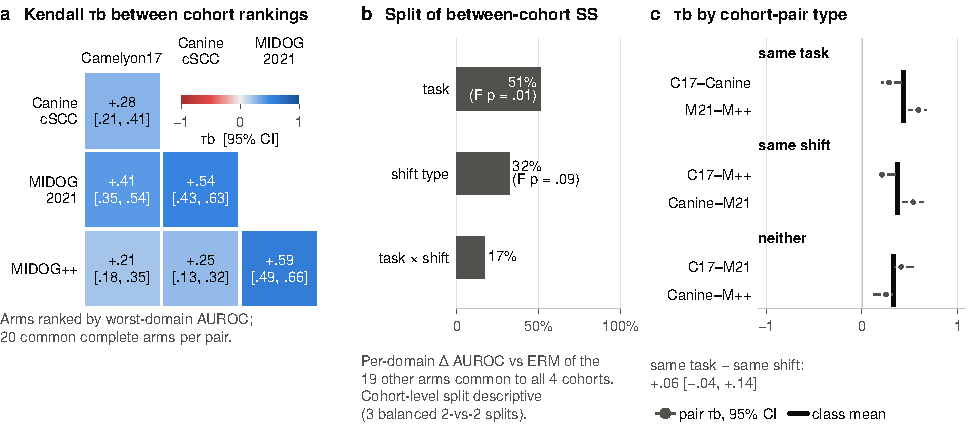
\includegraphics[width=\linewidth]{fig_kendall_C}
  \caption{Agreement of rankings between cohorts at the standard tier (top) and
  the compact tier (bottom). (a) Kendall's $\tau_b$ of worst-domain rankings
  with 95\% seed-bootstrap intervals. (b) Split of the between-cohort sum of
  squares of the per-domain gains over ERM into task, shift type and their
  interaction (Eq.~\ref{eq:2x2}); descriptive, since only three two-versus-two
  splits exist. (c) $\tau_b$ by type of cohort pair.}
  \label{fig:kendall}
\end{figure}

\subsection{Sensitivity analyses}
\label{sec:results-sensitivity}

\paragraph{Model-selection rule} Table~\ref{tab:selection} compares the
worst-domain ranking under each rule with the ID-validation ranking. At the
standard tier, the rules agree closely ($\tau_b$ 0.83--0.99), and the top arm
is the same under every rule on Camelyon17 and MIDOG++. At the compact tier,
agreement is weaker where run noise is large. On the canine cohort,
$\tau_b$ is 0.38 for OOD-validation selection and 0.32 for the oracle, and on
Camelyon17 it is 0.53--0.63. A compact-tier ranking thus depends on the
selection rule as well as on the seeds (Supplementary Fig.~\ref{S-fig:selection-C}).

\begin{table}[width=\linewidth,pos=t]
\caption{Agreement between model-selection rules: Kendall's $\tau_b$ between
the worst-domain ranking under each rule and the ranking under ID-validation
selection, over the arms analyzed under every rule (TTA pseudo-arms are
evaluated only under ID-validation selection). MIDOG~2021 has no OOD-validation
domain. Same top arm: whether every rule puts the same arm first.}
\label{tab:selection}
\footnotesize
% generated by src/v2/paper_tables.py from summary_{id,ood,last,oracle}.csv (worst-domain AUROC)
\begin{tabular*}{\tblwidth}{@{\extracolsep{\fill}}llrrrrl@{}}
\toprule
Tier & Cohort & Arms & $\tau_b$ OOD-val & $\tau_b$ last & $\tau_b$ oracle & Same top arm \\
\midrule
S & Camelyon17 & 20 & 0.84 & 0.83 & 0.85 & yes \\
 & Canine cSCC & 20 & 0.89 & 0.97 & 0.87 & no \\
 & MIDOG 2021 & 20 & -- & 0.85 & 0.85 & no \\
 & MIDOG++ & 20 & 0.97 & 0.99 & 0.96 & yes \\
\addlinespace[3pt]
C & Camelyon17 & 16 & 0.58 & 0.63 & 0.53 & no \\
 & Canine cSCC & 16 & 0.38 & 0.90 & 0.32 & yes \\
 & MIDOG 2021 & 16 & -- & 0.92 & 0.85 & yes \\
 & MIDOG++ & 16 & 1.00 & 1.00 & 0.98 & yes \\
\bottomrule
\end{tabular*}

\end{table}

\paragraph{Scale normalization of MIDOG~2021} Without normalizing the
$\approx$11\% difference in scanner magnification, the compact-tier ranking of
20 arms changes little ($\tau_b=0.78$ for the worst domain and 0.83 for the
mean). No arm's worst-domain AUROC moves by more than 0.039 (Supplementary
Fig.~\ref{S-fig:sensitivity}).

\paragraph{PatchCamelyon} Camelyon17 models were also scored on the
PatchCamelyon test split. PatchCamelyon comes from Camelyon16, whose two
hospitals also contribute to Camelyon17
\citep{veeling2018pcam,litjens2018camelyon}, so it is a secondary check, not an
independent cohort. At the standard tier the Lunit models,
fine-tuned or frozen, score highest, led by fine-tuned DINO with H\&E jitter
(mean over folds 0.908, against 0.772 for ERM). At the compact tier TIA-style
(0.802) and the augmentation arms score highest, against 0.698 for ERM
(Supplementary Table~\ref{S-tab:pcam}).

\paragraph{Calibration} On every cohort at the standard tier, one of the two
fine-tuned foundation models with H\&E jitter has the lowest mean ECE
(0.027--0.095), against
0.089--0.180 for ERM (Supplementary Fig.~\ref{S-fig:calibration-S}). Per-slide
normalization with jitter (TIA-style) and jitter alone are close: on the
canine cohort, their ECE is 0.075 and 0.080 at the standard tier and 0.047 and
0.065 at the compact tier.

\paragraph{Frozen representations} Among nine frozen backbones under one
linear-probe protocol (Supplementary Fig.~\ref{S-fig:ladder}), the Lunit Barlow Twins
ResNet-50 has the best worst-domain AUROC averaged over cohorts (0.841),
followed by the Lunit DINO ViT-S/16 (0.822). Pathology pre-training is not
enough by itself, however. The Lunit SwAV (0.707) and MoCo~v2 (0.734)
ResNet-50s are below ImageNet ConvNeXt-T (0.780) and ViT-B/16 (0.774), and
SwAV is below even the ImageNet ResNet-50 (0.718).

\subsection{The site acceptance test}
\label{sec:results-sat}

Figure~\ref{fig:sat} and Table~\ref{tab:sat} report the validation of the
site acceptance test of Section~\ref{sec:sat} over the 1,200 standard-tier
runs, with every held-out site playing the new site in turn. The development
prior alone is not a safe basis for a decision. Without local labels it
accepted 8.6\% of the sites whose true AUROC was below 0.80, because a model
that works at the development sites can still fail at a new one.

With local labels, the test kept false acceptance at or below 2.1\% for every
target and sample size, and at or below 1.3\% for sites more than 0.02 AUROC
below the target. Its 90\% credible intervals covered the true site AUROC in
92--93\% of cases. For targets of 0.80 and 0.85 it needed about half as many labels as local
labels alone. At a target of 0.80, it accepted 75\% of the good sites with 50 labels and 84\% with
100, while local labels alone accepted 48\% and 70\% and needed 200 labels to
reach 84\%. At a target of 0.85, the test reached with 100 labels (63\%) what
local labels alone reached with 200. Its point estimates were also more
accurate, with a mean absolute error of 0.024 AUROC at 50 labels against 0.036.
The price is a slightly higher false-acceptance rate than local labels alone,
by about one percentage point at the lower targets. The gain is largest where
the development sites score well above the target, as on Camelyon17 and
MIDOG++. Where they score near or below it, as on the canine cohort and at the
compact tier, the prior is pessimistic and can make the test less powerful
than local labels alone (Supplementary Table~\ref{S-tab:sat-cohorts}).

The advantage has limits. At the strict target of 0.90 with 200 or more
labels, local labels alone were slightly more permissive (55\% against 52\%
accepted at 200 labels). In the hardest subgroup, Camelyon17 at a target of
0.90, where most runs score above 0.95 and the 24 runs below the target mostly
fall just short of it, false acceptance reached 8.7\% with 25 labels and 5.7\%
with 50, and fell to 3.3\% at 100 and 1.7\% at 200. An $\epsilon$-contaminated
prior, which gives 10\% of the prior mass to a vague component centered at an
AUROC of 0.5, lowered these values to 5.4\%, 4.5\% and 2.8\%, at a cost in power
at small samples (for example from 38\% to 28\% at 25 labels and a target of
0.85; Supplementary Section~\ref{S-sup:sat}). We added this variant after
seeing the subgroup result and report it as a sensitivity analysis. At the
compact tier, whose sites score lower and differ more, the test was as safe
(false acceptance at most 0.4\%), but it gained over local labels alone only
at small samples and lost some power at larger ones. The decision threshold $1-\alpha$ is a posterior probability, so these
false-acceptance rates are empirical averages over the mix of bad sites in the
study, not a guaranteed error rate; for runs just below the target (within
0.02) false acceptance was higher, up to 5.8\% (target 0.80, 50 labels). The
label planner was close to the observed acceptance at the compact tier and
slightly optimistic at the standard tier, where it predicted 75\% acceptance of good
sites at 100 labels against 68\% observed.

\begin{figure}[pos=tbp]
  \centering
  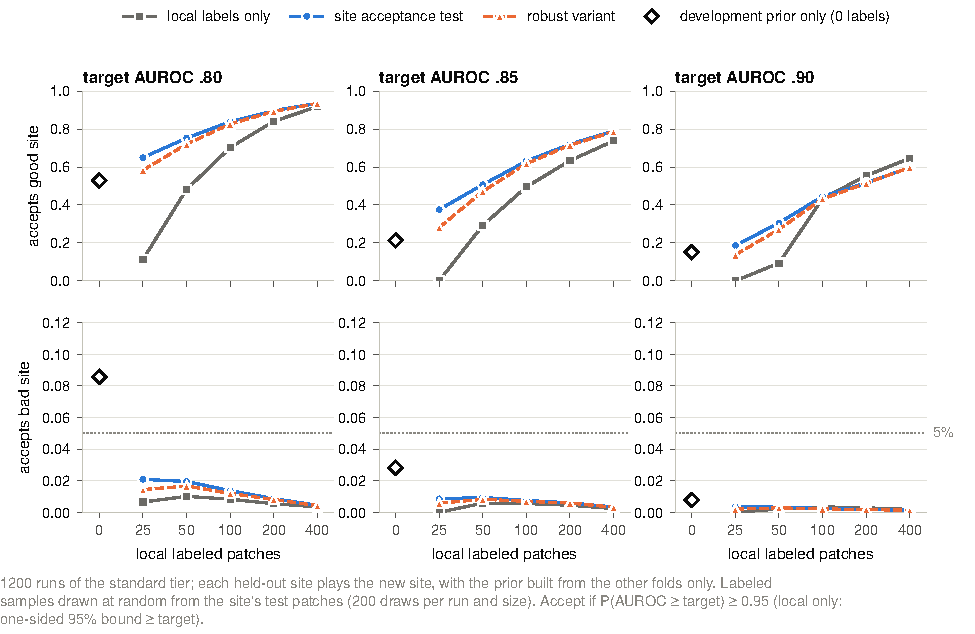
\includegraphics[width=\linewidth]{fig_sat_S}
  \caption{Validation of the site acceptance test at the standard tier.
  Top: share of good sites (true AUROC $\ge$ target) that each rule accepts;
  bottom: share of bad sites (true AUROC $<$ target) that it accepts, with the
  5\% level dotted. Means over runs of the acceptance rate over 200 random
  labeled samples per run and sample size. The compact tier is in
  Supplementary Fig.~\ref{S-fig:sat-C}.}
  \label{fig:sat}
\end{figure}

\begin{table}[width=\linewidth,pos=tbp]
\caption{Site acceptance test at the standard tier (1,200 runs). FA: false
acceptance, the percentage of runs with true site AUROC below the target $T$
that are accepted; power: the percentage of runs at or above $T$ that are
accepted; $m$: local labeled patches; MAE: mean absolute error of the point
estimate of the site AUROC; cover.: coverage of the 90\% interval. Rule: accept
if $P(\text{AUROC}\ge T)\ge0.95$ (local labels only: one-sided 95\% Wald bound
$\ge T$). The compact tier and the robust variant are in Supplementary
Section~\ref{S-sup:sat}.}
\label{tab:sat}
\footnotesize
\setlength{\tabcolsep}{3pt}
% generated by src/v2/site_acceptance.py tables (results/v2/site_acceptance/sat_rows_*.csv)
\begin{tabular*}{\tblwidth}{@{\extracolsep{\fill}}lrrrrrrrrr@{}}
\toprule
 & & \multicolumn{2}{c}{$T=0.80$} & \multicolumn{2}{c}{$T=0.85$} & \multicolumn{2}{c}{$T=0.90$} & & \\
\cmidrule(lr){3-4}\cmidrule(lr){5-6}\cmidrule(lr){7-8}
Rule & $m$ & FA (\%) & power (\%) & FA (\%) & power (\%) & FA (\%) & power (\%) & MAE & cover. (\%) \\
\midrule
Development prior only & 0 & 8.6 & 53 & 2.8 & 21 & 0.8 & 15 & -- & -- \\
\addlinespace[2pt]
Site acceptance test & 25 & 2.1 & 65 & 0.8 & 38 & 0.3 & 19 & 0.029 & 92 \\
 & 50 & 2.0 & 75 & 0.9 & 51 & 0.3 & 31 & 0.024 & 92 \\
 & 100 & 1.4 & 84 & 0.8 & 63 & 0.2 & 44 & 0.019 & 92 \\
 & 200 & 0.9 & 90 & 0.6 & 72 & 0.2 & 52 & 0.015 & 92 \\
 & 400 & 0.4 & 94 & 0.3 & 79 & 0.1 & 60 & 0.011 & 93 \\
\addlinespace[2pt]
Local labels only & 25 & 0.7 & 11 & 0.0 & 0 & 0.0 & 0 & 0.051 & 94 \\
 & 50 & 1.0 & 48 & 0.6 & 29 & 0.2 & 9 & 0.036 & 94 \\
 & 100 & 0.8 & 70 & 0.6 & 50 & 0.3 & 43 & 0.025 & 93 \\
 & 200 & 0.5 & 84 & 0.4 & 63 & 0.3 & 55 & 0.017 & 93 \\
 & 400 & 0.4 & 92 & 0.2 & 74 & 0.2 & 65 & 0.012 & 94 \\
\bottomrule
\end{tabular*}

\end{table}

% Flush the Results floats before the Discussion.
\clearpage

%% Discussion (MedIA revision, v2 pipeline). Numbers are those of Section 5 (sections/results.tex);
%% the case studies (sections/case_study.tex) use v1 numbers, labeled as such.
\section{Discussion}
\label{sec:discussion}

\subsection{What a domain-complete, seed-replicated evaluation shows}
\label{sec:disc-summary}

Four findings stand out.

First, a held-out score is mostly a statement about the held-out domain. For
most arms, the domain explains most of the variance of a single run, and the
same method can score near chance at one scanner and above 0.9 at another
(Section~\ref{sec:results-domains}). The worst domain also differs between
methods. A result on one official test split therefore describes one domain,
and a different split could reverse a comparison.

Second, with three to seven domains, most differences between methods cannot
be resolved statistically. No standard-tier arm beats ERM after correcting for
multiple comparisons, even when its mean gain is 0.145 AUROC and it improves
every domain. On the tumor cohorts, gains are large but vary strongly between
domains, so between 7 and 53 domains would be needed to confirm a gain of 0.05. On the
mitosis cohorts, differences are measured precisely but are small. Adding seeds
does not fix this, because the domain-by-method interaction dominates. This
agrees with DomainBed, where no algorithm beat ERM by a margin the authors
found significant \citep{gulrajani2021domainbed}, and with the large ERM seed
variance reported for Camelyon17 in WILDS \citep{koh2021wilds}.

Third, rankings are uncertain within a cohort and change between cohorts. At
the standard tier they agree more between cohorts that share a task than
between cohorts that share a shift type. This reverses the thesis of our own
earlier version, which held that the type of shift decides which method works
best. That thesis rested on two cohorts that differed in task as well as in
shift type, and the factorial design was built to separate the two. With four
cohorts, one per cell, the design can describe the pattern but cannot prove it,
and the compact tier does not clearly show it. We read the result as a warning,
not a law. A method's rank on one task says little about its rank on another,
even when the shift looks similar.

Fourth, implementation and tuning move results as much as the choice of
method. Estimating the stain matrix per tile instead of per slide turned the
fourth-best compact-tier arm on Camelyon17 into the worst. Inheriting a learning rate tuned
for another initialization made Barlow Twins fine-tuning fail on MIDOG++. The
defects that we found in our own earlier pipeline (Section~\ref{sec:casestudy})
are of the same kind. A comparison of methods is only as good as the weakest
implementation in it.

The method-level results are consistent with earlier work. Under the primary selection rule, none of the six
domain-generalization objectives ranked in the top five on any cohort. This is
consistent with DomainBed and WILDS, where such objectives did not reliably
beat ERM \citep{gulrajani2021domainbed,koh2021wilds}. Color
augmentation was consistently good, as \citet{tellez2019stain} found for HSV
and HED augmentation. Pathology foundation models were strong on the tumor
cohorts, but their frozen features were weak for mitotic figures, and two of
the four Lunit backbones were weaker frozen encoders than ImageNet ConvNeXt-T.
Domain-aligned pre-training beats ImageNet pre-training on average
\citep{kang2023benchmarking}, but which method helps varies across datasets and
shifts \citep{wiles2022fine}, and in our data it also varied with the task.

\subsection{A roadmap for models that work across sites without retraining}
\label{sec:roadmap}

Every number in this study answers a practical question: how well does a
model trained once on some sites work at a site it has never seen? No model
was trained on labeled data from its test site, and apart from the test-time
adaptation arms, no model was changed at all. The study therefore
doubles as a test of the ``train once, deploy at many sites'' strategy that
practitioners want. At the standard scale, the best method of each cohort
reached a worst-site AUROC of 0.884 to 0.986 without any retraining, against
0.534 to 0.895 for ERM. No single method was best everywhere, and no
improvement over ERM could be confirmed statistically with the sites
available. A practitioner can therefore improve the odds that a model
transfers, and can find out whether it does, but cannot assume it.

Figure~\ref{fig:roadmap} and Table~\ref{tab:roadmap} turn the results into six
steps. Each step carries an evidence grade. \emph{Strong} means that the
finding holds in all four cohorts at the standard tier. \emph{Moderate} means a
consistent direction that is not significant after correction, or a result
that holds with exceptions. \emph{Mixed}
means large gains in some cohorts and none in others. Step~6 uses the site acceptance test proposed in
Section~\ref{sec:sat}.

\begin{figure}[pos=tbp]
  \centering
  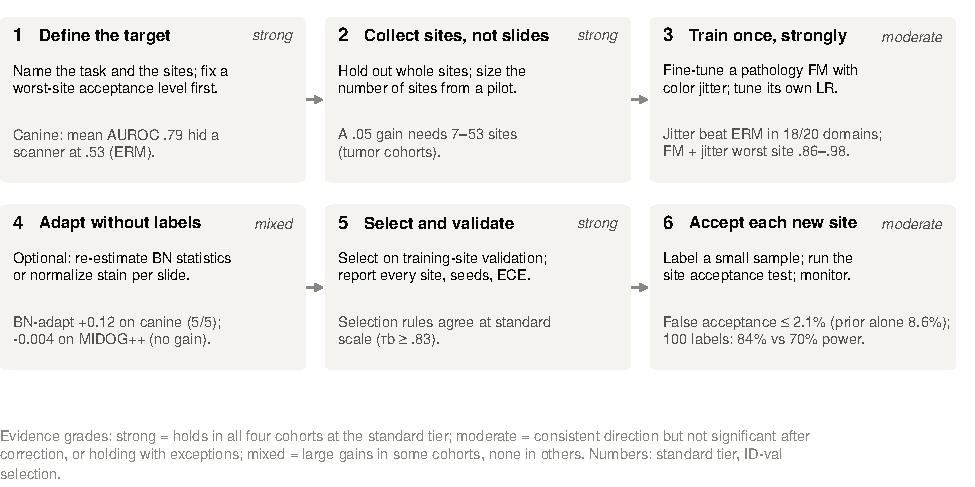
\includegraphics[width=\linewidth]{fig_roadmap}
  \caption{A six-step roadmap for pathology models that should work at new
  sites without retraining, with the evidence for each step from this study
  (standard tier, ID-validation selection) and its evidence grade. Details are
  in Table~\ref{tab:roadmap}.}
  \label{fig:roadmap}
\end{figure}

\paragraph{Step 1: define the target before training} Decide which task,
which sites and which scanners the model is meant for, and fix the minimum
performance that every site must reach. Judge models by their worst site.
Averages hid a near-chance scanner on the canine cohort (mean AUROC 0.785,
worst scanner 0.534 for ERM), and the hardest site differed between methods.

\paragraph{Step 2: collect sites, not only slides} Gather development data
from as many sites and scanners as possible, and split it by site. Most of the
variance of a held-out score comes from the site (median ICC 0.72--0.95), so
extra slides or extra training runs from the same sites do little. A pilot
study gives $\sigma_\Delta$, and Eq.~\eqref{eq:power} then says how many sites
a validation needs. In our tumor cohorts, confirming a gain of 0.05 AUROC
needed 7 to 53 sites.

\paragraph{Step 3: train once, with a strong recipe} Start from a pathology
foundation model, fine-tune it end to end with H\&E color jitter, and tune the
learning rate for that initialization. In our data, color jitter improved mean
AUROC over ERM in 18 of 20 held-out domains at the standard tier, and the
fine-tuned DINO ViT with jitter had the best worst-site AUROC averaged over
the four cohorts (0.895). Two warnings apply. Frozen foundation-model features
were not enough for mitotic figures (the frozen probes ranked 18th to 21st on
both mitosis cohorts), so frozen features must be checked on the task at hand.
And an initialization with the wrong learning rate can fail outright: Barlow
Twins fine-tuning with the ImageNet learning rate reached 0.715 mean AUROC on
MIDOG++, against 0.891 with its own rate. Domain-generalization objectives
deserve low priority; under the primary selection rule, none of the six
reached the top five on any cohort.

\paragraph{Step 4: adapt to the new site without labels, if the pipeline
allows it} Two techniques need neither labels nor any change to the trained
weights. They use only unlabeled images of the new site at prediction time.
Re-estimating the batch-normalization statistics (BN-adapt) helped most where
the shift was severe. At the standard tier it raised mean AUROC by 0.120 on the
canine scanners, at all five of them, and by 0.015 and 0.022 on Camelyon17 and
MIDOG~2021, but it did nothing on MIDOG++ ($-0.004$). Per-slide stain
normalization gave smaller gains than color jitter in three of the four
cohorts at the standard tier. Both
techniques must be implemented with care. The test images must arrive in
shuffled, mixed batches, because a batch of one class corrupts the statistics
(Section~\ref{sec:setup-arms}). Stain must be estimated from enough tissue: a
per-tile estimate failed at a whole Camelyon17 center (0.557 against 0.976 for
the per-slide estimate; Supplementary Section~\ref{S-app:macenko}). TENT, by contrast,
updates model parameters at test time and is thus a form of fine-tuning.

\paragraph{Step 5: select and validate without touching the target sites}
Choose hyperparameters and checkpoints on held-out data from the training
sites only. Validate by holding out whole sites in turn with at least three
seeds per model. Report every site, the worst site, the seed spread, the
calibration at each site and confidence intervals that account for the
training data shared between folds. At the standard scale, the choice of
selection rule barely changed the rankings ($\tau_b\ge0.83$). With the small
compact model it did ($\tau_b$ down to 0.32), which is one more reason not to
draw conclusions from toy models. Calibration also varies: on Camelyon17 alone,
the mean ECE of standard-tier methods ranged from 0.027 to 0.186.

\paragraph{Step 6: accept each new site with a small labeled sample, then
monitor} Before a model is used at a new site, label a small random sample of
that site's patches, spread over many slides, and run the site acceptance test
of Section~\ref{sec:sat} against the target of Step~1. The development results
of Step~5 supply its prior, and its planner gives the number of labels to
collect. At the standard tier, the test kept false acceptance at or below 2.1\%
and, for targets of 0.80 and 0.85, needed about half as many labels as local
labels alone. The development
results alone were not enough: they would have accepted 8.6\% of the sites
that fell below a target of 0.80. Where the development sites score far above the
target, a site that fails is a surprise to the prior, so at least 100 labels
should be collected; the robust variant, which we added after seeing this
case, lowers the risk further. Where they score near or below the target, the
prior adds little and local labels decide. After acceptance, inputs and outputs
should be monitored; we did not test monitoring.

\begin{table}[width=\linewidth,pos=tbp]
\caption{The roadmap of Fig.~\ref{fig:roadmap} with its evidence. Numbers are
standard-tier results under ID-validation selection unless stated. Grades:
strong, holds in all four cohorts at the standard tier; moderate, consistent
direction but not significant after correction, or holding with exceptions;
mixed, large gains in some cohorts and none in others.}
\label{tab:roadmap}
\footnotesize
\begin{tabular*}{\tblwidth}{@{\extracolsep{\fill}}>{\raggedright\arraybackslash}p{2.1cm}>{\raggedright\arraybackslash}p{5.2cm}>{\raggedright\arraybackslash}p{6.2cm}l@{}}
\toprule
Step & What to do & Evidence in this study & Grade \\
\midrule
1. Define the target & Fix the task, sites, scanners and a worst-site acceptance level before training. & Canine ERM: mean 0.785, worst scanner 0.534; the worst site differed between methods (Sec.~\ref{sec:results-domains}). & strong \\
2. Collect sites & Split by site; size the number of sites from a pilot estimate of $\sigma_\Delta$. & Median ICC 0.72--0.95; a 0.05 gain needs 7--53 sites (tumor) or 3 (mitosis); extra seeds help little (Sec.~\ref{sec:results-variance}, \ref{sec:results-contrasts}). & strong \\
3. Train once, strongly & Fine-tune a pathology foundation model with H\&E jitter; tune its own learning rate; check frozen features on the task; give DG objectives low priority. & Jitter better than ERM in 18/20 domains; DINO FT + jitter best mean worst-site AUROC (0.895); frozen probes 18th--21st on mitosis; BT with inherited learning rate 0.715 vs 0.891 on MIDOG++; no DG objective in the top five (Sec.~\ref{sec:results-ranks}). & moderate \\
4. Adapt without labels & Optionally re-estimate BN statistics on shuffled site images, or normalize stain per slide; never per small tile. & BN-adapt $+0.120$ on canine (5/5 scanners), $+0.015$ and $+0.022$ on Camelyon17 and MIDOG~2021, $-0.004$ on MIDOG++; per-tile Macenko 0.557 vs 0.976 per slide at one center (Suppl.~\ref{S-app:macenko}). & mixed \\
5. Select and validate & Select on training-site data; hold out whole sites with $\ge$3 seeds; report every site, the worst site, seeds, ECE and intervals. & Selection rules agree at the standard tier ($\tau_b\ge0.83$) but not at the compact tier (down to 0.32); ECE 0.027--0.186 on Camelyon17 (Sec.~\ref{sec:results-sensitivity}). & strong \\
6. Accept each new site & Label a small random sample; accept if the site acceptance test gives $P(\text{AUROC}\ge T)\ge0.95$; plan $m$ with its planner; monitor afterwards. & Development results alone: 8.6\% false acceptance at $T=0.80$. Test: false acceptance $\le$2.1\%; at $T=0.80$, 84\% power with 100 labels, which local labels alone need 200 for; worst subgroup 8.7\% and 5.7\% with 25 and 50 labels, 3.3\% with 100 (Sec.~\ref{sec:results-sat}). Monitoring not tested. & moderate \\
\bottomrule
\end{tabular*}
\end{table}

\paragraph{What the roadmap does not promise} It does not guarantee that a
model will work at a new site; it raises the chance, measures the risk and
checks each site before use. Its
evidence comes from patch classifiers at 96 to 224~px on four public research
cohorts, not from whole-slide or detection systems in clinical use, and clinical
deployment additionally needs prospective and regulatory validation that this
study does not provide. The method choices in Step~3 were the best on average,
not on every cohort, which is exactly why Steps 5 and 6 cannot be skipped.

\subsection{What method developers should report}
\label{sec:disc-research}

For researchers who propose or compare methods, the results add five reporting
rules to the roadmap. Each one changed a conclusion in this study.
\begin{enumerate}
  \item \emph{Report every domain and repeat runs.} A single official split is
    one sample from a wide distribution, and the seeds of one method spanned
    up to 0.48 AUROC at a single domain.
  \item \emph{Report intervals and power.} State $\sigma_\Delta$ and the
    number of domains a claimed gain would need, treat a large non-significant
    gain as unresolved, and account for the training data that folds share
    \citep{nadeau2003inference,bates2023cv}.
  \item \emph{Include controls and tune every method.} On MIDOG++,
    compute-matched ERM was the best compact-tier arm and well ahead of
    SimCLR, which passes the same number of images through the encoder; on
    the canine cohort it was the worst. Without the control, neither result
    could be attributed correctly.
  \item \emph{Report all model-selection rules, and separate transductive
    methods.} Methods that use unlabeled test-site images were among the
    strongest and should be compared with each other.
  \item \emph{Do not transfer rankings across tasks, and release per-run
    records.} Cohorts that shared only the shift type ranked methods almost
    independently at the standard tier, and stored records let others add
    rules and metrics without retraining.
\end{enumerate}

%% Case study (withdrawn v1 synergy claim) and the NCT-CRC-HE scope result.
%% All numbers are from the authors' earlier (v1) pipeline, recomputed from:
%%   runs/camelyon17_center2/*.json, results/camelyon17_center2/*.csv
%%   $DATA/runs/fold{0..4}/{baseline,sam,ssl,ssl_sam}_seed{0,1,2}.json (ood_test.auroc)
%%   results/nct_crc_he/crc_results_summary.csv, crc_results_raw.csv,
%%   crc_interaction.csv, crc_data_manifest.json
%% v1 arm names: baseline = ERM, ssl = SimCLR, sam = SAM, ssl_sam = SimCLR+SAM.
%% v2 interaction: results/v2/analysis/paper_numbers.json -> simclr_sam_interaction_C (from C/*/per_run_id.csv).

\subsection{Case study: a single-hospital synergy claim that did not survive}
\label{sec:casestudy}

This study began with a claim of our own that the protocol of
Section~\ref{sec:protocol} overturns. The numbers below come from our earlier
(v1) pipeline: a compact CNN on 64~px crops, five epochs and selection on the
OOD-validation hospital, not the v2 protocol.

\paragraph{The original claim} The model was trained on Camelyon17 hospitals 0,
3 and 4, selected on hospital 1 and tested on hospital 2, the official WILDS
split \citep{koh2021wilds}. With one seed per arm, test AUROC was 0.931 for
ERM, 0.895 for SimCLR, 0.826 for SAM and 0.951 for SimCLR+SAM. The interaction
$I=\delta_{\text{SimCLR+SAM}}-\delta_{\text{SimCLR}}-\delta_{\text{SAM}}$, with
$\delta$ the difference from ERM, was $+0.161$ ($\delta_{\text{SimCLR}}=-0.037$,
$\delta_{\text{SAM}}=-0.105$, $\delta_{\text{SimCLR+SAM}}=+0.019$). Each method
alone was worse than ERM and the pair was better, so we read $I$ as a synergy.
Patch-bootstrap intervals were narrow (SAM$-$ERM:
$[-0.108,-0.102]$).

\paragraph{What the design got wrong} The patch bootstrap measures test
sampling, not run-to-run variation. A second ERM seed in the same experiment
scored 0.881, 0.050 below the first and about 15 times the half-width of that
interval. With both available seeds for ERM and SimCLR, $I$ falls to $+0.112$.
As a contrast of four single runs, $I$ carries the run noise of all four arms.

\paragraph{How the protocol detects it} The v1 grid has all five hospitals and
three seeds per cell (fold $t$ tests on hospital $t$). At hospital 2, $I$ is
$-0.019$. Over hospitals 0--4 it is $-0.012$, $-0.012$, $-0.019$, $+0.180$ and
$-0.050$: negative at four of five, with mean $+0.017$ (95\% CI
$[-0.097,+0.132]$, $p=0.70$, Eq.~\ref{eq:mean}). The single positive value
comes from one SAM run at hospital 3 with test AUROC 0.407 (other seeds:
0.908 and 0.864). At hospital 2, the seed SDs of ERM, SAM,
SimCLR and SimCLR+SAM (0.105, 0.065, 0.048 and 0.002) give a single-run SD of $I$ of about 0.13
if run noise is independent across arms, so $+0.161$ is about 1.2 SDs from
zero. Seed replication thus shows that one run cannot separate the effect from
noise, and domain completeness that its sign depends on the test hospital.
We withdraw the synergy claim. Under the v2 protocol (compact tier, five
seeds per arm, ID-validation selection), the interaction on Camelyon17 is
$-0.003$, $-0.007$, $+0.066$, $+0.007$ and $+0.057$ at hospitals 0--4, with
mean $+0.024$ (95\% CI $[-0.019,+0.067]$, $p=0.20$). On the other cohorts it is
$-0.007$ (canine), $-0.013$ (MIDOG~2021) and $+0.003$ (MIDOG++). Under v2, the
official test hospital shows the largest positive value ($+0.066$). A
single-hospital study on that split would again report a synergy that the full
design does not support. The small negative value on MIDOG~2021 (95\% CI
$[-0.021,-0.005]$, unadjusted $p=0.02$, $K=3$) is the only interval that
excludes zero.

\paragraph{Validity of the v1 records} The v1 defects documented in this
revision (MixStyle active at evaluation, Macenko as one fixed color transform,
RotInv identical to ERM, inactive IRM annealing, an empty GroupDRO group on
MIDOG~2021 and the canine cohort, TENT on single-class test batches) do not
touch these four arms. One deviation does apply: v1 SAM updated batch-norm running statistics on the
perturbed pass instead of the unperturbed one, the reverse of the standard
implementation, and v2 corrects it. It affects SAM and SimCLR+SAM in both
v1 experiments, by an amount we have not measured. The single-hospital
experiment also used an earlier script and a different 30,000-patch training
sample than the grid, so its values are not interchangeable with fold~2's.

\subsection{A single-institution cohort cannot support domain claims (NCT-CRC-HE)}
\label{sec:nct}

We also ran the four v1 arms on NCT-CRC-HE-100K \citep{kather2018nct}, with
two seeds each. The task was tumor epithelium versus all other tissue except
background, on the central $64\times64$~px of each tile. Training (20,000
tiles), ID validation (4,000) and the SimCLR pool (10,226 unlabeled tiles)
came from the color-normalized release. There were two test conditions: the
same release without color normalization (4,000 tiles), and CRC-VAL-HE-7K
\citep{kather2019predicting}, which comes from 50 other patients of the same
tissue bank (class-balanced to 2,466 tiles).

\paragraph{$K=1$ by construction} The tiles have no site labels, so no domain
can be held out. The cohort is one domain, and model selection had to use ID
validation. Neither test condition changes the institution.

\paragraph{Result} All arms reach ID-validation AUROC of 0.963--0.972 (means
over two seeds). Without color normalization, ERM scores 0.791, SAM 0.726,
SimCLR+SAM 0.724 and SimCLR 0.702 ($-0.089$ relative to ERM). On CRC-VAL-HE-7K
the four arms span only 0.017 (0.927--0.944). ERM has the lowest ECE in both
test conditions (0.157 against 0.206--0.235, and 0.027 against 0.032--0.037).
Note that SimCLR's pool saw only normalized tissue, so it never saw the
un-normalized appearance it was tested on.

The arithmetic of Section~\ref{sec:casestudy} recurs. Without normalization,
both single methods are worse than ERM, and $I=+0.087$. A tile bootstrap of
the two-seed ensembles gives $+0.078$ $[0.070,0.085]$. That interval reflects
tile sampling only, while SimCLR's two seeds differ by 0.102 in the same
condition (0.752 and 0.651).

\paragraph{Why this is a scope statement} With $K=1$ there are no
leave-one-domain-out folds and no between-domain variance $\sigma_D$ or ICC
(Eq.~\ref{eq:oneway}). Eq.~\ref{eq:mean} also needs $K\ge2$. The result shows
that, on one tissue source, SimCLR pre-trained on normalized tiles did not
help under an unseen stain appearance or on new patients. It says nothing
about institutional shift either way. We report it to set the scope of our conclusions. The SAM
batch-norm caveat above applies here too.


\subsection{Limitations}
\label{sec:limitations}

\paragraph{Four cohorts, one per cell} The task-by-shift analysis has one
cohort per cell. Task, species, tissue, label definition and training-set size
vary together between cells, and the cohort-level decomposition is
descriptive. The two mitosis cohorts share MIDOG~2021's 150 images. More
cohorts per cell would be needed to separate task from shift type
statistically.

\paragraph{Few domains} With $K=3$ to 7, the ICC and the paired contrasts have
wide intervals, and fold dependence can only be handled as a sensitivity
analysis. MIDOG~2021 has no OOD-validation domain.

\paragraph{Model scale and input size} The standard tier uses ResNet-50 at
96~px and ViT-S/16 at 224~px. Patch classification at this size is not
whole-slide inference or mitotic-figure detection, and larger inputs or
detection pipelines may rank methods differently. The two tiers already
disagree in part (Section~\ref{sec:results-ranks}).

\paragraph{Foundation models} HuggingFace was not reachable from our compute
environment, so recent large foundation models such as UNI, Virchow or
Prov-GigaPath \citep{chen2024uni,vorontsov2024virchow,xu2024gigapath} were not
evaluated. The Lunit models are trained on TCGA only and are licensed for
non-commercial research.

\paragraph{Tuning} Hyperparameters were tuned with one seed per fold, and the
compact tier uses a fixed learning rate. Some selected values lie at a grid
edge (Supplementary Section~\ref{S-app:tuning}). A larger search could change individual
ranks.

\paragraph{Transductive stain normalization} Per-slide Macenko normalization
estimates each test slide's stain from that slide's benchmark patches, which
were sampled from annotated regions. The effect of this tile set on the
estimate was small (Supplementary Section~\ref{S-app:macenko}), but a label-independent tissue
sample would match practice better.

\paragraph{Secondary cohorts} PatchCamelyon overlaps with Camelyon17 in its
hospitals, and NCT-CRC-HE has no site labels, so neither tests institutional
shift. The case studies use numbers from our earlier pipeline, which differs
from the v2 protocol.

\paragraph{Site acceptance test} The test assumes that a new site is
exchangeable with the development sites, so a site unlike all of them must be
caught by the local labels; in the hardest subgroup it needed 100 labels to
keep false acceptance below 5\%. It was validated on labeled patches drawn at
random from each site's test patches, whereas real labels come in clusters from
a few slides, which widens the local uncertainty. It addresses patch-level
AUROC, not a clinical endpoint, and its label planner was slightly optimistic
at the standard tier.

\paragraph{Metric} AUROC is the primary metric. It ignores the decision
threshold, which matters in practice, and threshold-dependent metrics may
rank methods differently. They are stored in every record.

%% Conclusion (MedIA revision, v2 pipeline).
\section{Conclusion}
\label{sec:conclusion}

We asked whether pathology models can be trained once and then used at new
hospitals and scanners without retraining, and how a practitioner can tell.
Holding out every domain of four public cohorts, repeating every run and
selecting models without test data, we found that the train-once strategy can
work well: the best standard-scale method of each cohort kept a worst-site
AUROC between 0.88 and 0.99 without seeing labels from the test site. It is
not guaranteed, however. No method was best on every cohort, ERM fell to near
chance on one scanner, and with three to seven sites few differences between
methods could be confirmed, because most of the uncertainty comes from the
sites, not from the seeds.

Fine-tuned pathology foundation models with color augmentation were the most
reliable recipe on average, and color augmentation alone was close behind.
Re-estimating batch-normalization statistics on unlabeled images of the new
site helped mainly under severe scanner shift. Under the primary selection
rule, domain-generalization objectives never reached the top five, and frozen
foundation-model features were weak for mitotic figures. At the standard
scale, rankings agreed more between cohorts that share a task than between
cohorts that share a type of shift, so evidence from one task transfers poorly
to another.

Because development results cannot guarantee performance at a new site, we
proposed a site acceptance test that combines them with a small labeled sample
from that site. Validated on every held-out site, it kept false acceptance at
or below 2.1\% at standard scale and needed about half as many labels as local
labels alone, whereas the development results alone accepted 8.6\% of the
sites that fell below an AUROC of 0.80.

The roadmap of Section~\ref{sec:roadmap} turns these results into six steps:
define a worst-site target, collect many sites, train once with a strong
recipe, adapt without labels where the pipeline allows it, validate by holding
out whole sites, and accept each new site with the site acceptance test. The
protocol, the diagnostics and all per-run records are released so that other
cohorts and methods can be added to the same analysis.


%%% ---------------------------- Appendices --------------------------
%%% (lettered; equations, figures and tables numbered A.1, B.1, ...)
%%% Supplementary material: separate file supplementary.tex (cross-references via xr, prefix S-).

%%% ---------------------------- Back matter (MedIA order) -----------
%%% CRediT is printed from the \credit{} entries above.
\printcredits

\section*{Declaration of competing interest}
% MedIA also requires the Elsevier declaration-tool .docx at the Attach Files
% step (see submission/declarations_checklist.md); its text must match this one.
The authors declare that they have no known competing financial interests or
personal relationships that could have appeared to influence the work reported
in this paper.

\section*{Funding}
This research did not receive any specific grant from funding agencies in the
public, commercial, or not-for-profit sectors.

\section*{Data and code availability}
All data used in this study are public. Camelyon17-WILDS
\citep{koh2021wilds,bandi2019camelyon17} and PatchCamelyon
\citep{veeling2018pcam} are released under CC0~1.0. NCT-CRC-HE-100K and
CRC-VAL-HE-7K \citetext{\citealp{kather2018nct,kather2019predicting};
Zenodo, \doilink{10.5281/zenodo.1214456}} are released under CC~BY~4.0. The MIDOG~2021 training
set \citetext{\citealp{aubreville2023midog}; Zenodo,
\doilink{10.5281/zenodo.4643381}} and the multi-scanner canine cutaneous
squamous cell carcinoma cohort \citetext{\citealp{wilm2023canine}; Zenodo,
\doilink{10.5281/zenodo.7418555}} are released under CC~BY~4.0. MIDOG++ \citetext{\citealp{aubreville2023midogpp}; figshare,
\doilink{10.6084/m9.figshare.c.6615571.v1}} is publicly available; the collection record is licensed
CC~BY~4.0 and its constituent image and label files CC0~1.0. The pretrained
pathology weights of \citet{kang2023benchmarking} (ResNet-50 Barlow Twins,
SwAV and MoCo~v2; ViT-S/16 DINO) were obtained from
\url{https://github.com/lunit-io/benchmark-ssl-pathology} and are used under
the Lunit Inc.\ Public License, which permits non-commercial research use only.
The ImageNet-1k weights of the ResNet, ConvNeXt and ViT backbones are the
torchvision defaults, and the SWAG ViT-B/16 weights \citep{singh2022swag},
also obtained through torchvision, are released under CC~BY-NC~4.0
(non-commercial use).
Code, the fold-materialization scripts for all cohorts, the per-run records
of every job, the variance-decomposition, interval and power code, and the
script that regenerates every table and figure from those records are
available at \coderepo.
The release contains the records of all 4,778 runs and the test-set
predictions of every final run, from which the site acceptance test is
validated.
\todoauthors{archive the release on Zenodo and cite the code as software with
its DOI.}

\section*{Acknowledgements}
\todoauthors{acknowledgements (computing resources, colleagues), or delete
this section.}

%%% Elsevier: placed at the end of the core manuscript, immediately above the
%%% references (hence after the Acknowledgements).
\section*{Declaration of generative AI and AI-assisted technologies in the writing process}
% TODO-AUTHORS: confirm the tool and the reason (Elsevier wording, do not paraphrase).
During the preparation of this work the authors used Claude (Anthropic) in
order to assist with code review, analysis scripting, drafting of the
manuscript text and language editing.
After using this tool/service, the authors reviewed and edited the content as
needed and take full responsibility for the content of the publication.
\todoauthors{confirm}

%%% ---------------------------- References --------------------------
\bibliographystyle{cas-model2-names}
\bibliography{main}

%%% Author vitae (<= 100 words each) go in a separate editable file for MedIA;
%%% the CAS \bio environment is available if the editors want them inline.
%\bio{}
%\endbio

\end{document}
